%%%%%%%%%%%%%%%%%%%%%%%%%%%%%%%%%%%%%%%%%%%%%%%%%%%%%%%%%%%%%%%%%%%%%%
%%  
%%  UT-THESIS.TEX
%%
%% This program can be redistributed and/or modified under the terms
%% of the LaTeX Project Public License Distributed from CTAN archives
%% in directory CTAN:/macros/latex/base/lppl.txt.
%%
%%  Copyright (c) 1999 by Francois Pitt
%%  Last Update: 1999 May 13
%%  
%%%%%%%%%%%%%%%%%%%%%%%%%%%%%%%%%%%%%%%%%%%%%%%%%%%%%%%%%%%%%%%%%%%%%%
%%  
%%  This file is distributed in the hope that it will be useful but
%%  without any warranty (without even the implied warranty of
%%  fitness for a particular purpose).  For a description of this
%%  file's purpose, and instructions on its use, see below.
%%  
%%  Feel free to copy and redistribute this file, as long as this
%%  copyright notice remains intact and this file is distributed
%%  along with the companion file `ut-thesis.cls'.
%%  
%%  (Thanks to Robert Bernecky for his suggestions on improving the
%%  usefulness and readability of this file.)
%%  
%%  Send all bugs, questions, comments, suggestions, etc. to the
%%  author, at <fpitt@cs.utoronto.ca>.
%%  
%%%%%%%%%%%%%%%%%%%%%%%%%%%%%%%%%%%%%%%%%%%%%%%%%%%%%%%%%%%%%%%%%%%%%%
%%  
%%  Skeleton LaTeX2e file for the preparation of theses at UofT;
%%  conforms to the School of Graduate Studies' guidelines of 07/97.
%%  To be used in conjunction with class file `ut-thesis.cls', whose
%%  features it illustrates.
%%  
%%  To comment out parts of a file, use the macro \ignore{...}
%%  around the entire block of text you want to ignore.
%%  
%%  To explicitly set the pagestyle of any inserted blank page when
%%  \cleardoublepage occurs, use one of \clearemptydoublepage or
%%  \clearplaindoublepage instead.
%%  
%%  For single-spaced quotes or quotations, use the `longquote' and
%%  `longquotation' environments.  For single-spaced, 1 1/2-spaced,
%%  or double-spaced paragraphs, use one of the environments
%%  `singlespaced', `oneandahalfspaced', or `doublespaced'.  More
%%  generally, for paragraphs with a line spacing of `n', use
%%  `\begin{newspacing}{n}...\end{newspacing}'.
%%  
%%  All other environments, commands, and options provided by the
%%  `ut-thesis' class will be described below, at the point where
%%  they should appear in the document.
%%  
%%  See the companion file `ut-thesis.cls' for more details.
%%  
%%%%%%%%%%%%%%%%%%%%%%%%%%%%%%%%%%%%%%%%%%%%%%%%%%%%%%%%%%%%%%%%%%%%%%


%%%%%%%%%%%%         PREAMBLE         %%%%%%%%%%%%

%% Default settings format a final copy (12pt font, single-sided,
%% double-spaced, normal margins, single-spaced notes).  For a rough
%% copy (10pt font, double-sided, double-spaced, normal margins, with
%% the word "DRAFT" printed at each corner of every page), use the
%% `draft' option.  The default line spacing can be changed with one
%% of the following options: `singlespaced', `oneandahalfspaced', or
%% `doublespaced'.  The notes are always single-spaced by default, but
%% can be made to have the same spacing as the rest of the document by
%% using the option `spacednotes'.  The size of the margins can be
%% changed with one of the following options: `narrowmargins' (1 1/4"
%% left, 3/4" others), `normalmargins' (1 1/4" left, 1" others),
%% `widemargins' (1 1/4" all), `extrawidemargins' (1 1/2" all).  Any
%% other standard option for the `report' document class can be used
%% to override the default or draft settings.

%% ***   Add any desired options.   ***
\documentclass{ut-thesis}

%% ***   Add \usepackage declarations here.   ***


%% The line spacing of the document should be specified using one of
%% the document options given above, but if you need a line spacing
%% that is not provided by the options, you can override the default
%% line spacing for the entire document with the command
%%   `\linespacing{...}'.
%% Note that in order to get the correct appearance, the argument to
%% `\linespacing' must be equal to 1/3 + 2/3 times the desired line
%% spacing (for example, single-spaced = \linespacing{1},
%%                        1 1/2-spaced = \linespacing{1.33}, and
%%                       double-spaced = \linespacing{1.66}).

%% ***   Uncomment and fill in a value, if needed.    ***
%% ***   REMEMBER: You should NOT need to use this.  Use one of   ***
%% ***   the document class options mentionned above instead.     ***
%\linespacing{}

%%%%%%%%%%%%%%%%%%%%%%%%%%%%%%%%%%%%%%%%%%%%%%%%%%%%%%%%%%%%%%%%%%%%%%
%%                                                                  %%
%%                  ***   I M P O R T A N T   ***                   %%
%%                                                                  %%
%%  Fill in the following fields with the required information:     %%
%%   - \degree{...}       name of the degree obtained               %%
%%   - \department{...}   name of the graduate department           %%
%%   - \gradyear{...}     year of graduation                        %%
%%   - \author{...}       name of the author                        %%
%%   - \title{...}        title of the thesis                       %%
%%%%%%%%%%%%%%%%%%%%%%%%%%%%%%%%%%%%%%%%%%%%%%%%%%%%%%%%%%%%%%%%%%%%%%

%% ***   Change this example to appropriate values.   ***
\degree{Doctor of Philosophy}
\department{Biochemistry}
\gradyear{2012}
\author{Grace Li}
\title{Molecular mechanism of amyloid inhibition and protein denaturation}

%% ***   NOTE   ***
%% Put here all other formatting commands that belong in the preamble.


%% For example, to list only down to subsections in table of contents
%% (-1=part, 0=chapter, 1=section, 2=subsection, 3=subsubsection,
%%  4=paragraph, 5=subparagraph, 6=subsubparagraph).
%
\setcounter{tocdepth}{2}


%%%%%%%%%%%%      MAIN  DOCUMENT      %%%%%%%%%%%%

\begin{document}

%% ***   NOTE   ***
%% You should put all of your `\newcommand', `\newenvironment', and
%% `\newtheorem's (in other words, all the global definitions that
%% you will need throughout your thesis) in a separate file and use
%% "\input{filename}" to input it here.


%% This sets the page style and numbering for preliminary sections.
\begin{preliminary}

%% This generates the title page from the information given above.
\maketitle

%% There should be NOTHING between the title page and abstract.

%% This generates the abstract page, with the line spacing adjusted
%% according to SGS guidelines.
\begin{abstract}
%% ***   Put your Abstract here.   ***
%% (At most 150 words for M.Sc. or 350 words for Ph.D.)
% TODO: This is my Biophysical society abstract.  MUST REWORD and readapt
Alzheimer's disease (AD) is a severe neurodegenerative disease with no cure. Currently, one method of targeting the underlying disease is to prevent or reverse the amyloid formation of A$\beta$42, a key pathological hallmark of AD. A small-molecule novel drug candidate, Scyllo-inositol, is a polyol small-molecule that exhibits stereochemistry dependent inhibition of the formation of fibrils in vitro.  Furthermore, recently completed phase II clinical trials demonstrated that scyllo-inositol achieved target drug levels in the cerebral spinal fluid (CSF) of Alzheimer’s patients, a main challenge for AD drug candidates to to overcome. 
Despite its promise as a therapeutic for AD, the mechanism of action of scyllo-inositol at the molecular level is currently not understood.  We perform extensive microsecond timescale atomistic explicit solvent molecular dynamics simulations of scyllo-inositol and its inactive stereoisomer, chiro-inositol with the full length A$\beta$42 protofibril.  From our simulations, we predict binding affinities and characterize the binding modes of inositol and their stereochemistry-dependent effect on the structure of A$\beta$42 protofibrils.  Our results provide molecular insight for the rational design of small-molecule inhibitors of A$\beta$42 and other amyloid-based diseases.
\end{abstract}

%% Anything placed between the abstract and table of contents will
%% appear on a separate page since the abstract ends with \newpage
%% and the table of contents starts with \clearpage.

%% This generates a "dedication" section, if needed.
%% (uncomment to have it appear in the document)
\begin{dedication}
This thesis is dedicated to my grandparents, and my mother.
\end{dedication}

%% The `dedication' and `acknowledgements' sections do not create new
%% pages so if you want the two sections to appear on separate pages,
%% you should put an explicit \newpage between them.
\newpage

%% This generates an "acknowledgements" section, if needed.
%% (uncomment to have it appear in the document)
\begin{acknowledgements}
	
First and foremost, I am grateful to my supervisor, Regis Pomes for his wisdom, insight, and guidance for the past 6 years of my life.

Secondly, I thank the members of my lab, both past and present, for all their moral support, and assistance with my work. 
I would like to thank the early members of the lab Drs. Chris Madill, Chris Neale, Sarah Rauscher and Tomas Rodinger for setting an example for me of how to be an excellent student of science. Not only were they brilliant scientists, they have provided the lab with invaluable insight, and technical expertise.

% advice and support which have had a profound influence on my perspective on life.
Nilu Chakrabarti, David Caplan, John Holyoake, Loan Huynh, Kethika K.

% Thank Mr. Zimmerman

% Thank Dr. Nasir Memon

% Thank SciNet & Team
% The computations presented in this thesis were resource intensive and I could not have accomplished any of it without generous allocations from the center for computational biology (CCB) at Sickkids and the following high-performance computing (HPC) consortia of Compute Canada: SciNet, SHARCNET, CLUMEQ, WestGrid, and RQCHP.
% My use of these computing resources was only possible because of the excellent support staff at each of these consortia. While there are perhaps one hundred people who have contributed to this thesis in this respect, I would like to mention some of those people who have provided exceptional levels of support.

Finally, I thank my mom and my grandparents for all of their support over the years. Without them I would not be here today.

\end{acknowledgements}

%% This generates the Table of Contents (on a separate page).
% \tableofcontents

%% This generates the List of Tables (on a separate page), if needed.
%% (uncomment to have it appear in the document)
% \listoftables

%% This generates the List of Figures (on a separate page), if needed.
%% (uncomment to have it appear in the document)
% \listoffigures

%% End of the preliminary sections: reset page style and numbering.
\end{preliminary}

%%%%%%%%%%%%%%%%%%%%%%%%%%%%%%%%%%%%%%%%%%%%%%%%%%%%%%%%%%%%%%%%%%%%%%
%%  Put your Chapters here; the easiest way to do this is to keep   %%
%%  each chapter in a separate file and `\include' all the files    %%
%%  right here.  Note that each chapter file should start with the  %%
%%  line "\chapter{ChapterName}".  Note that using `\include'       %%
%%  instead of `\input' makes each chapter start on a new page.     %%
%%%%%%%%%%%%%%%%%%%%%%%%%%%%%%%%%%%%%%%%%%%%%%%%%%%%%%%%%%%%%%%%%%%%%%

%% ***   Include chapter files here.   ***
\chapter{Introduction}

% Maybe start off as far back as "protein folding" ?
% What would I write though?
% Check out Misbehaving proteins the book.

% Broad theme: Protein folding, self-assembly, and its modulation ???
% Importance of protein folding -- structure - function paradigm
% Functions by binding with other proteins or ligands in the body.
% Ok, we also know about intrinsically disordered proteins that have well-defined functions in the human body.
% 
% But what about amyloid ... this common state that all proteins reach which results from protein aggregation

% The general problem of protein - structure and function
Perhaps one of the most remarkable phenomenon of nature is the ability of proteins to fold and self-assemble from a polypeptide chain into structures which impart their functions as molecular machines of life.

% Since the historical experiment performed by Anfinsen and colleagues which demonstrated that the structure of a folded protein is dependent on upon in its amino acid sequence and solvent environment, the protein folding problem has emerged as an important problem in biochemistry and biophysics.

% Protein interactions, and how protein function may be modulated by these interactions -- particularly solvent interactions.
Aenean orci erat, aliquet eu feugiat vitae, laoreet in justo. Aenean non dapibus leo. Pellentesque in nulla nec justo commodo varius ut congue ante. Aenean neque nibh, ornare sit amet tincidunt in, ullamcorper vitae risus. Aliquam rutrum porta suscipit. Aliquam erat volutpat. Aenean odio diam, vehicula sed interdum non, fringilla eu eros. Nunc ac diam arcu.


For many years, structural biologists focused their studies on proteins with well-defined folded states, and proteins capable of functioning without a unique folded state were largely sidelined.

% Protein misfolding and aggregation
However, in recent years, much attention have been focused on understanding what happens when proteins misfold, that is fail to achieve its proper folded structure necessary to carry out their normal physiological function.  Furthermore, the important of intrinsically disordered proteins, a class of proteins which do not adopt rigid 3-dimensional structures under physiological conditions, have gained much attention due to their roles in regulation, signaling.   Among these IDPs are a subset of proteins which are involved in numerous human diseases.  These proteins have been found to aggregate to form amyloid fibrils under certain solution conditions. Amyloid fibrils are widely known to be involved in many incurable diseases such as prion-related diseases, neurodegenerative diseases, Type II diabetes, and systemic amyloidosis. 


% It is also thought that amyloid fibrillar state may be the globally stable folded state for all proteins.

% Perhaps show a table here of all the proteins and diseases that they may be involved in.
% Columns Protein, has a structure?, disordered?, disease it is involved in.

\section{The amyloid state of proteins}
% A paragraph as a general introduction to amyloid.
% What's the general interest behind amyloid science -- why is amyloid important
% Here lead into a more detailed discussion about AD
% Role of amyloid in the human body

About 150 years ago, amyloids were defined as tissue deposits of extracellular filaments.\cite{Haass:2007db,Sipe:2000fs} These fibrillar deposits were microscopically visible, and sometimes even visible by eye in various organs in many seemingly unrelated human diseases.

Amyloid deposits all show specific optical behaviour (such as birefringence) on binding certain dye molecules such as Congo red.

% amyloid may be general to all proteins
The ability of polypeptide chains to form amyloid structures is not restricted to the relatively small number of proteins associated with recognized clinical disorders. Amyloid fibrils were observed to be formed in vitro by many other peptides and proteins, including well-known molecules such as myoglobin, and also by homopolymers such as polythreonine or polylysine.  
% This suggests that the amyloid state may be the globally stable for all polypeptides.

Although the ability of proteins to form amyloid fibrils appear to be generic, the propensity for a given peptide is highly dependent on the formation condition, and vary for different sequences. 

% The relative aggregation rates for a wide range of peptides and proteins correlates with the physicochemical features of the molecules such as charge, secondary-structure propensities and hydrophobicity. 

In a globular protein the polypeptide main chain and the hydrophobic side chains are largely buried within the folded structure. Only when they are exposed, for example when the protein is partly unfolded (for example, at low pH) or fragmented (for example, by proteolysis), will conversion into amyloid fibrils be possible. 


% How is amyloid formed
% kinetics of aggregation ?
Amyloid fibrils are formed via a complex aggregation pathway. Initially, monomers aggregate to form oligomers with different morphologies which exists in equilibrium with amyloid fibrils. Some of these oligomers are on-pathway to fibril formation, while others themselves may be end-points of the aggregation pathway. Biochemically, fibrils are protease resistant and are insoluble in the presence of Sodium dodecyl sulfate (SDS).


Amyloid fibrils have been observed to form via a two-step nucleation-polymerization process, a behaviour that is typical of nucleated processes such as crystallization.  In the nucleation phase, a lag phase occurs where energetic barriers of aggregation must be overcome to form the initial aggregation nucleus. Seeding, a process where preformed aggregates is introduced into solutions, may eliminate the lag phase.  Following the lag phase, free monomers may bind to the nucleated aggregates and polymerize into mature fibrils.\cite{Murphy:2002fe} 


\subsection{Fibrils}

\begin{figure}
  \centering
  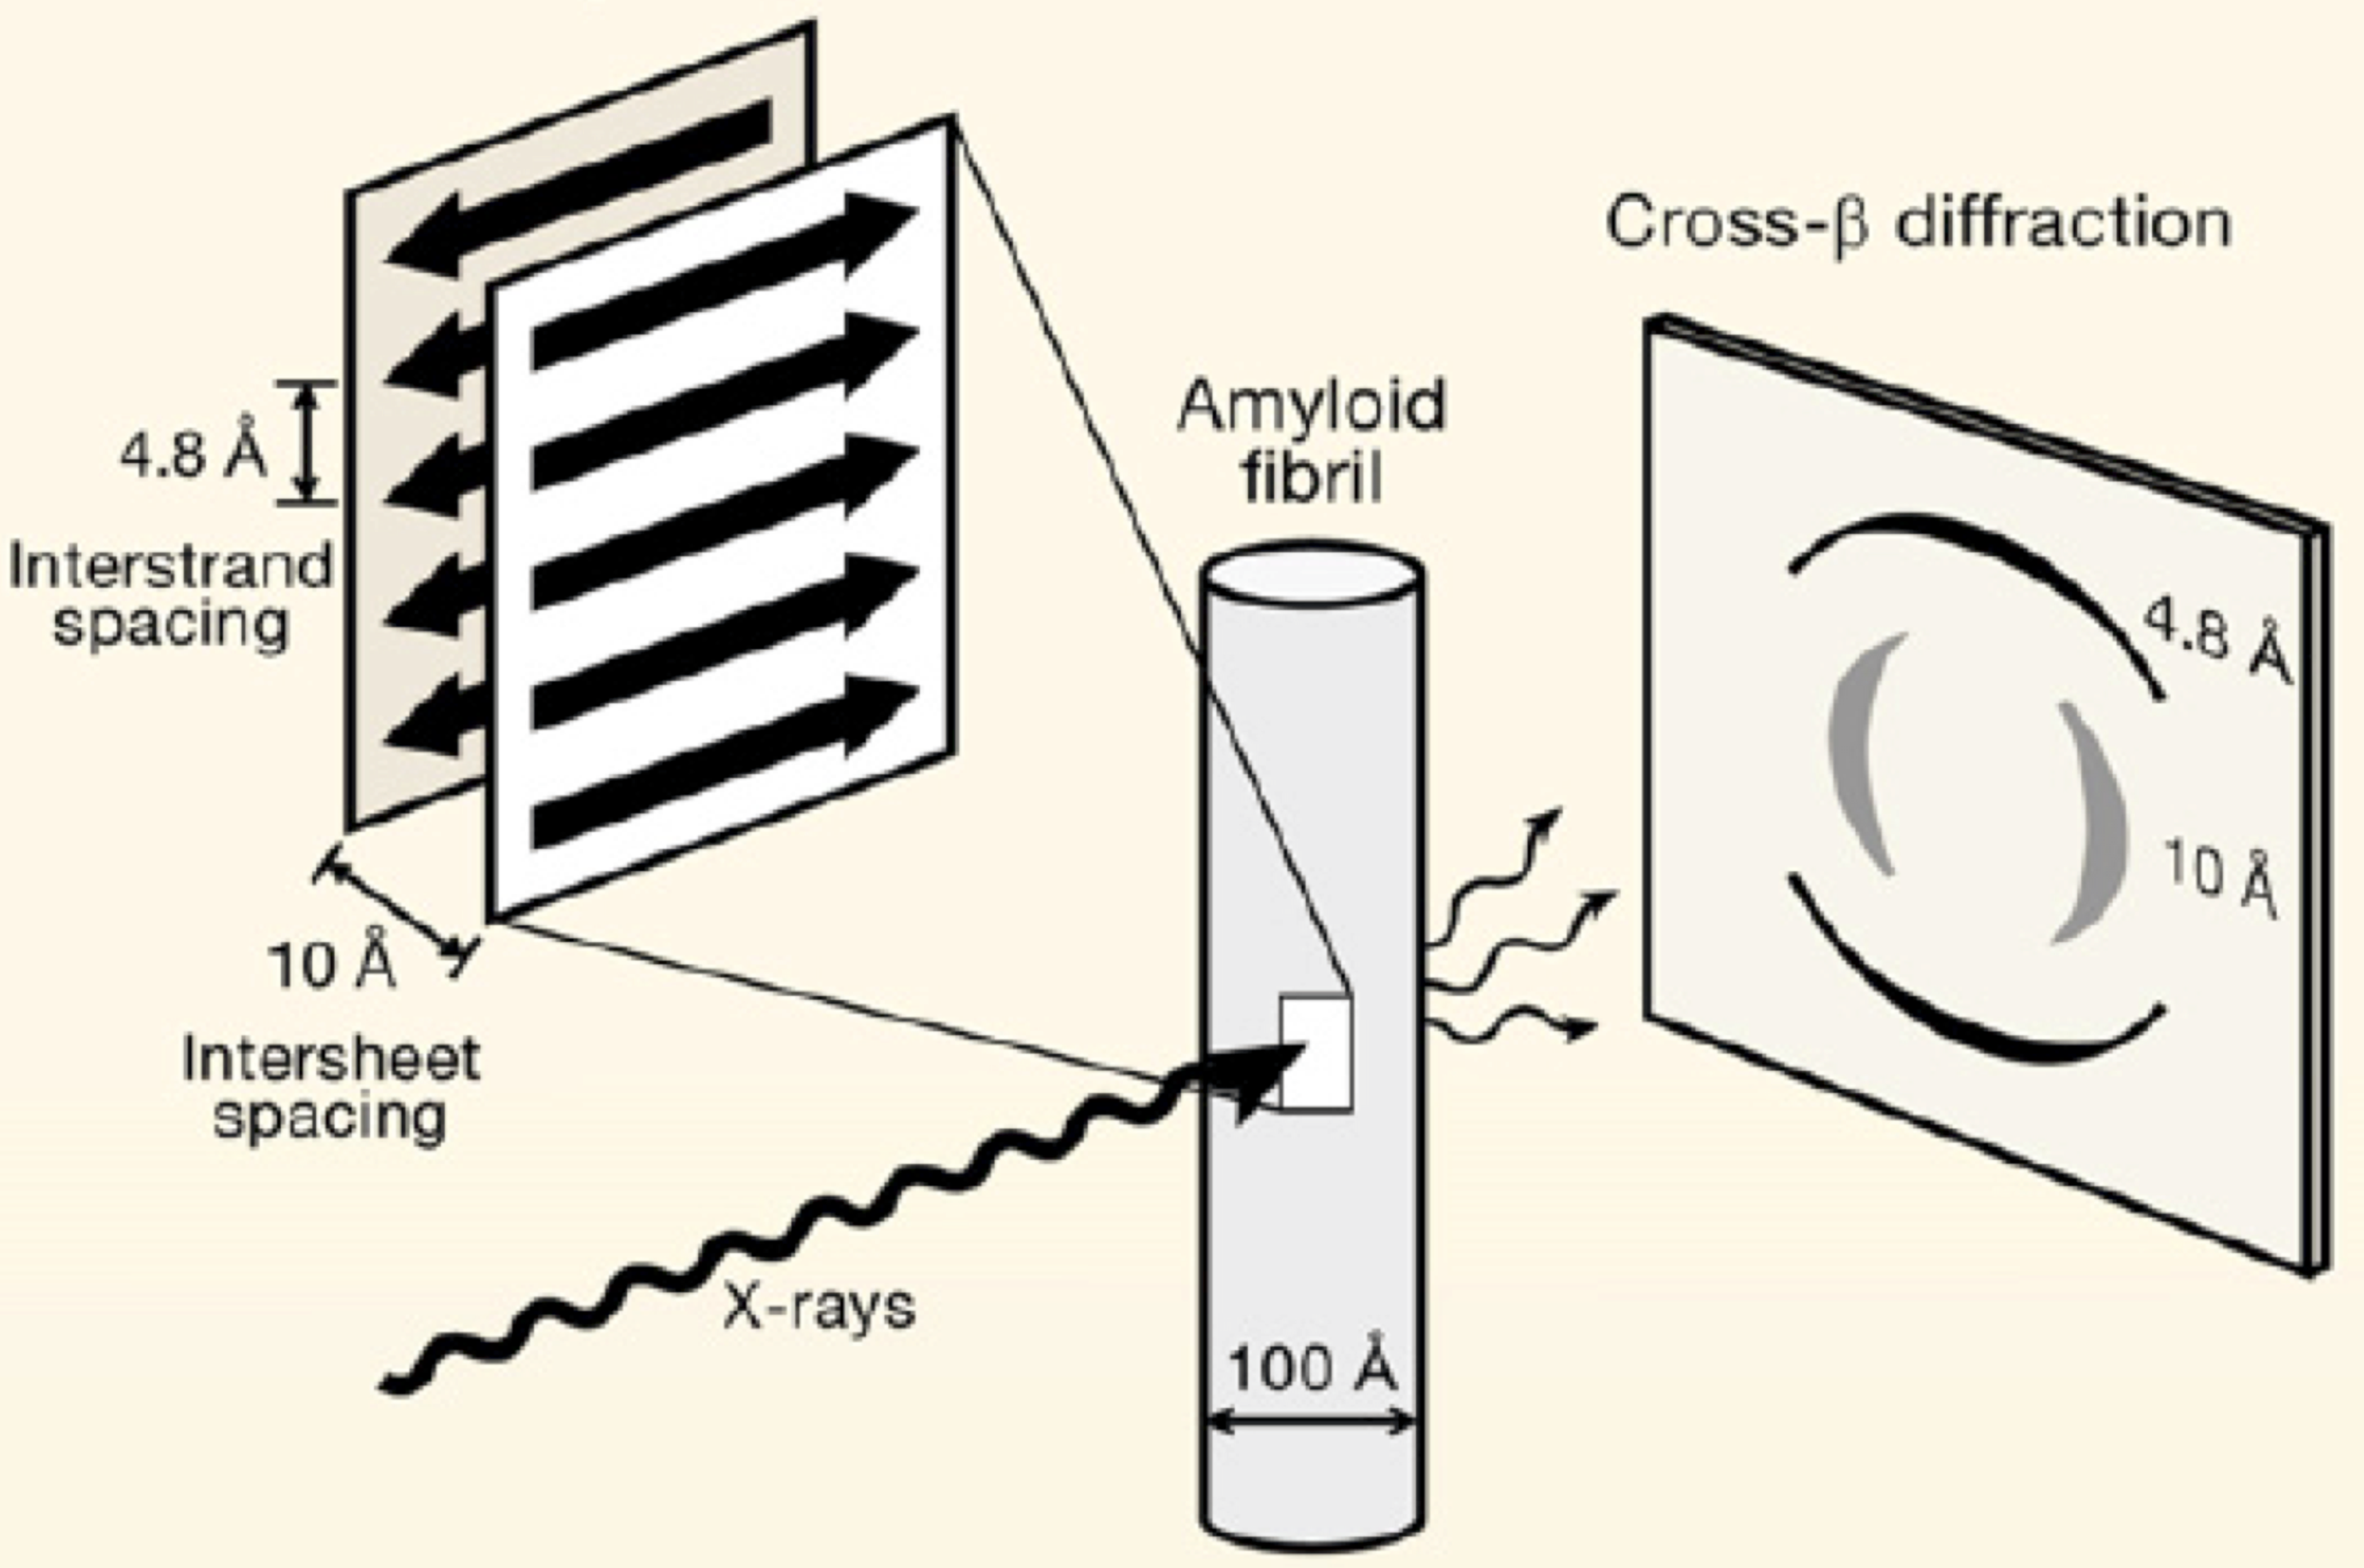
\includegraphics[width=6in]{figures/introduction/fibril_structure_diffraction.pdf}
  \caption[Characteristic cross-$\beta$ spacings from X-ray fibre diffraction studies of amyloid fibrils]{This is adapted from Eisenberg, 2012}
  \label{fig:fibril_diffraction}
\end{figure}

% Finding a treatment for AD and other fatal neurodegenerative diseases motivated many biochemical and biophysical studies of the amyloid state. 

Despite having dramatically different sequences, amyloid fibrils formed from different polypeptide all adopt a similar structure called the \crossbs.  The first structural studies of fibrils using X-ray fiber diffraction showed that a \crossb\ is characterized by a 4.8\angstrom\ interpeptide, and 10\angstrom\ intersheet spacing. XXX add more details to this description. XXX [Need to have a figure which shows this diffraction pattern, and EM data with cartoon model.] This defining characteristic of \crossb\ have now been adopted by biophysicists as an indication for the presence of amyloid fibrils.


Under the transmission electron microscope (TEM), fibrillar structures typical of many aggregates are visible as long, unbranched, often twisted ribbon-like structures nanometers in diameter (Figure~\ref{fig:fibril_TEM_SSNMR}). Independent measurements of fibrillar structure using different instruments have all confirmed the presence of \crossbs as the core structure of amyloid fibrils. (Figure~\ref{fig:fibril_diffraction})

% Other measurements 
% MPL Mass per unit length

Although \crossb\ is widely known, due to the insolubility and inherent non-crystalline nature of amyloid fibrils, the details of the fibril structure at the molecular level remained elusive until recently. Advances in solid-state NMR (SSNMR) and X-ray crystallography in the last decade have made major contributions to our knowledge of the molecular structure of amyloid fibrils.

\begin{figure}
  \centering
  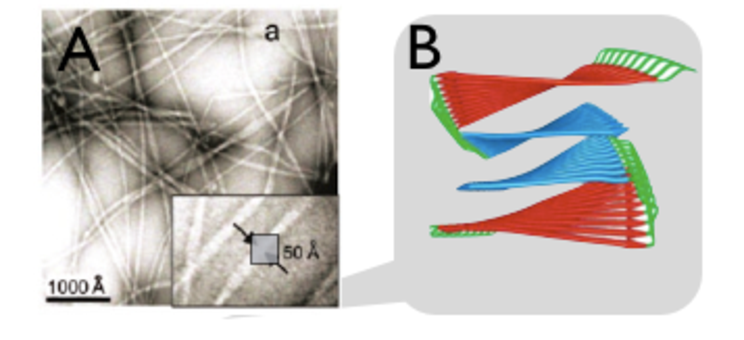
\includegraphics[width=6in]{figures/introduction/fibril_TEM_SSNMR.pdf}
  \caption[Characteristic cross-$\beta$ spacings from X-ray fibre diffraction studies of amyloid fibrils]{A Example EM images of oligomers.  Adapted from Bitan G. et al. 2003 and Walsh D. 1999 C TEM image of fibrils D SSNMR model proposed by Tycko et al.}
  \label{fig:fibril_TEM_SSNMR}
\end{figure}

% Describe the molecular structure of \abeta\ amyloid fibrils. 
% Briefly mention the techniques that can be used to obtain structural information of amyloid fibrils. 

% SSNMR
The initial molecular model of an amyloid fibril was for \abeta40, the peptide involved in Alzheimer's disease.  A SSNMR study on the amyloid fibrils of A$\beta$40 was done by Tycko et al in 2002. XXX The fibril core of \abeta40 involves the stretch sequence XXX-YYY. It is thought that residues A to B is disordered. The core fibril unit consists of a parallel in-register \bsheet, where each strand is a \bhairpin\ with peptide-peptide backbone hydrogen-bond along the long axis of the fibril. Figure~\ref{fig:fibril_TEM_SSNMR}


% X-ray structures
Furthermore, small peptide fragments that have characteristics of amyloid fibrils, which are also amenable to single crystal X-ray diffraction analysis have demonstrated similar type structures from those studied using SSNMR.  These structures obtained by X-ray crystallography have been described to have a dry interface with stacked sheets. (Figure~\ref{fig:fibril_xray_model})

\begin{figure}
  \centering
  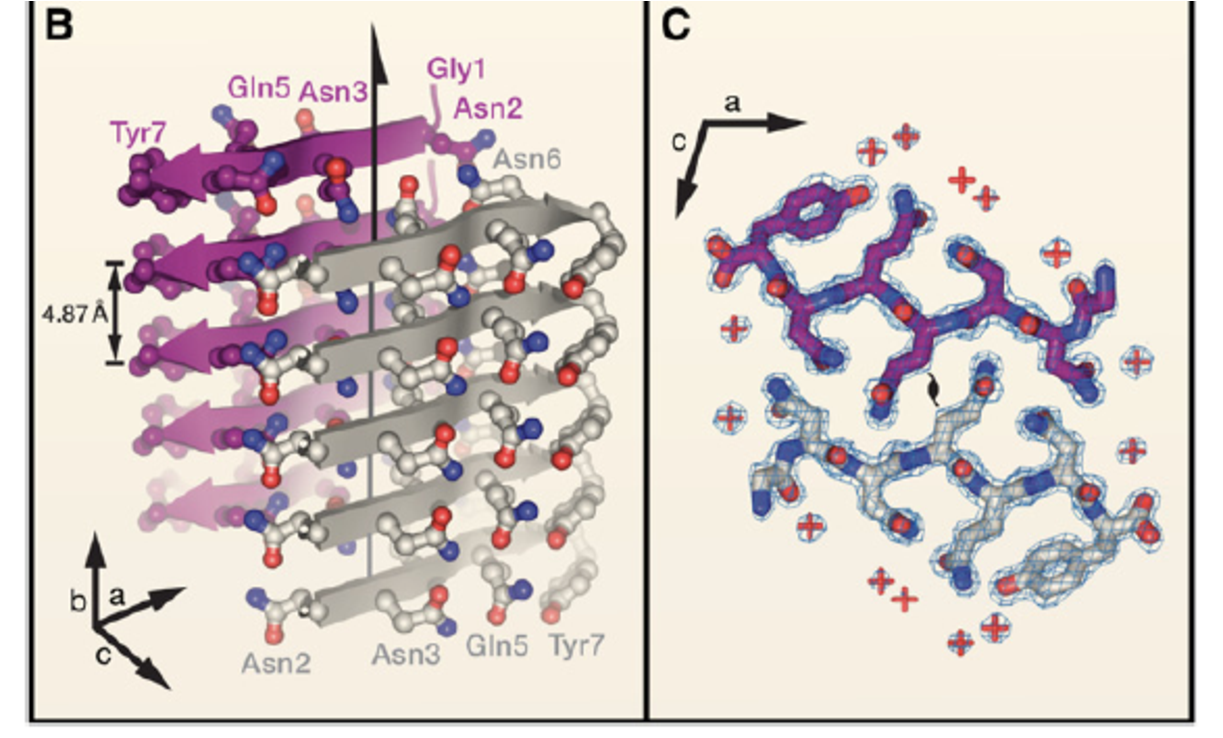
\includegraphics[width=6in]{figures/introduction/fibril_xray_model.pdf}
  \caption[Characteristic cross-$\beta$ spacings from X-ray fibre diffraction studies of amyloid fibrils]{This is adapted from Eisenberg, 2012}
  \label{fig:fibril_xray_model}
\end{figure}

% What do all fibrils have in common?
% Organization of the peptide backbone into beta-sheets; sheet stacking
The ubiquitous presence of a \crossbs supports that the organization of the peptidic backbone, common to all proteins, in to \bsheets\ is a major determinant of the fibrillar structure. Moreover, the proposed structures (some described above), indicate that the core region is composed of two to four sheets that interact closely with each other.

% I don't think I will talk about the twisting of the sheets too much.
% An interesting feature of these sheets is that they appear to be much less twisted than ex- pected from the analysis of the short arrays of β-strands that form β-sheets in globular protein structures. This feature was first proposed from cryo-EM and has been supported by Fourier transform infrared (FTIR) analy- ses (48, 61).

\subsection{Polymorphism of fibrils}

% Even fibrils formed from a single peptide can exhibit polymorphism .
Although all fibrils share the \crossbs, individual fibrils exhibit polymorphism at the molecular level which is dependent upon the experimental conditions under which they are formed.  % (Figure~\ref{fig:fibril_diffraction})
Fibrils may vary in the length of the beta-strand involved, side chain orientation. 

\subsection{Non-fibrillar oligomers}
\begin{figure}
  \centering
  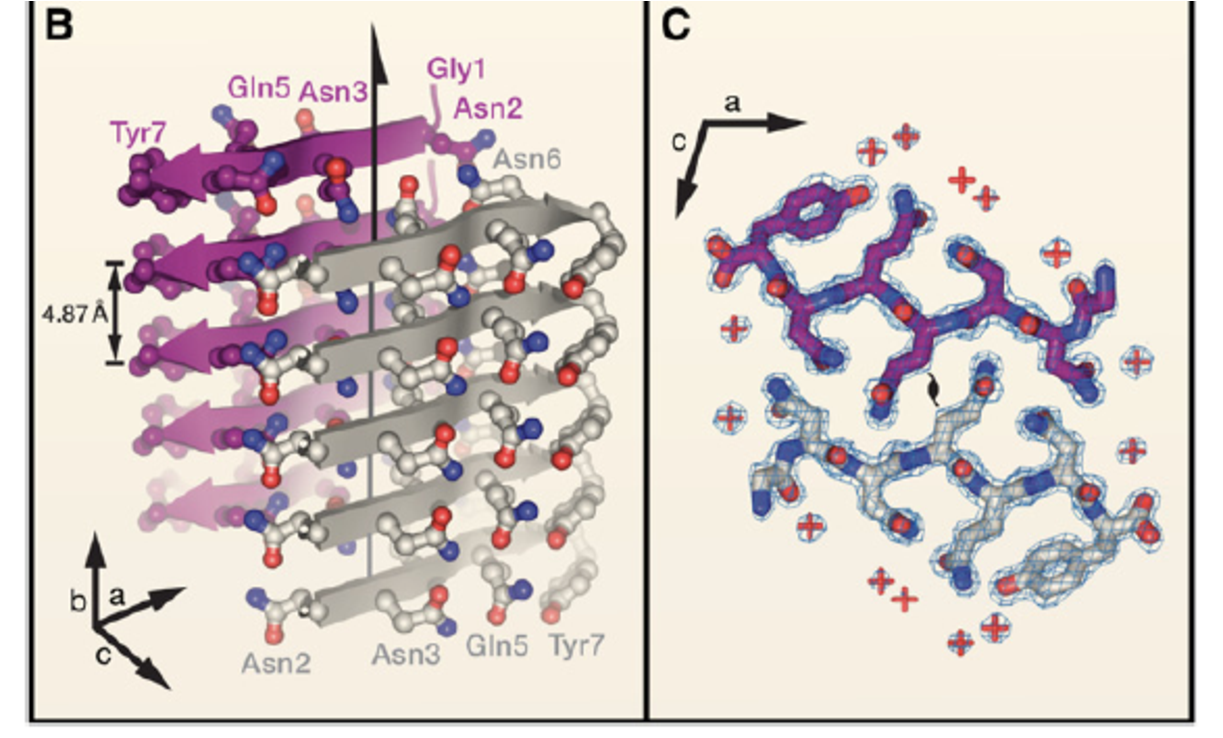
\includegraphics[width=6in]{figures/introduction/fibril_xray_model.pdf}
  \caption[Characteristic cross-$\beta$ spacings from X-ray fibre diffraction studies of amyloid fibrils]{This is adapted from Eisenberg, 2012}
  \label{fig:fibril_xray_model}
\end{figure}

Due to their structural disorder and their insolubility, molecular details of oligomers have been challenging to obtain using current structural determination techniques. 

EM and AFM experiments have shown that transient, unstable particles may appear prior to the formation of fibrils. In particular, soluble \abeta\ prefibrillar assemblies that are annular, spherical, or curvilinear in shape have been reported in literature.REF Protofibrils, in particular, are curvilinear, filamentous structures that are smaller than mature fibrils and are approximately 5-10 nm in diameter.9 Furthermore, protofibrils bind to dyes Thioflavin T (ThT) and Congo Red (CR), suggesting the presence of substantial β-sheet content.9, 13-15 Although some of these particles may be \bsheet-rich, they are morphologically distinct and are typically much smaller than fibrillar structures. Figure~\ref{fig:oligomers}

Despite the importance of these prefibrillar species in causing neurodegeneration, their molecular structures are still not known. However, a recent SSNMR study demonstrated that a late stage, neurotoxic Aβ40 spherical intermediate contained fibril-like β-sheet structure.16

[ Recent data show that non-fibrillar oligomers may contain fragments which are fibril-like in morphology. Most recently a study have shown that oligomers of \abeta\ ]
[ Should briefly read up on the book chapter by Pat Walsh]

\subsubsection{Amyloid Toxicity}
% I think outline some of the ideas / hypothesis about the link between amyloid and disease, but don't go into what people speculate or data on toxicity. It is related, but this is out of the scope of your thesis.

	% Key question in the field: What is the toxic species?
Multiple lines of research have identified oligomers as a likely causative agent for neuronal cell death. By contrast, the monomeric and fibril forms are thought to be less toxic than oligomers. It is hypothesized that soluble oligomers may cause toxicity by perturbing the integrity of cellular membranes through binding and disrupting the lipid bilayer (perhaps by making them ion permeable). \cite{Walsh:2007fu}

% Include a paragraph about amyloid formation and lipid membranes

% Understanding the toxicity or finding out whether there is a toxic species in part validates the amyloid hypothesis. 

% Here can lead into AD by saying well ... a widely known disease, where amyloid oligomers are thought to directly play a role in the disease process is AD.  

\section{Alzheimer's Disease}
One of the most well-known diseases involving amyloid formation is Alzheimer's Disease (AD), a devastating neurodegenerative disease that is most common cause of dementia in persons of age 65 or older.

% Pathological characterization
\begin{figure}
  \centering
  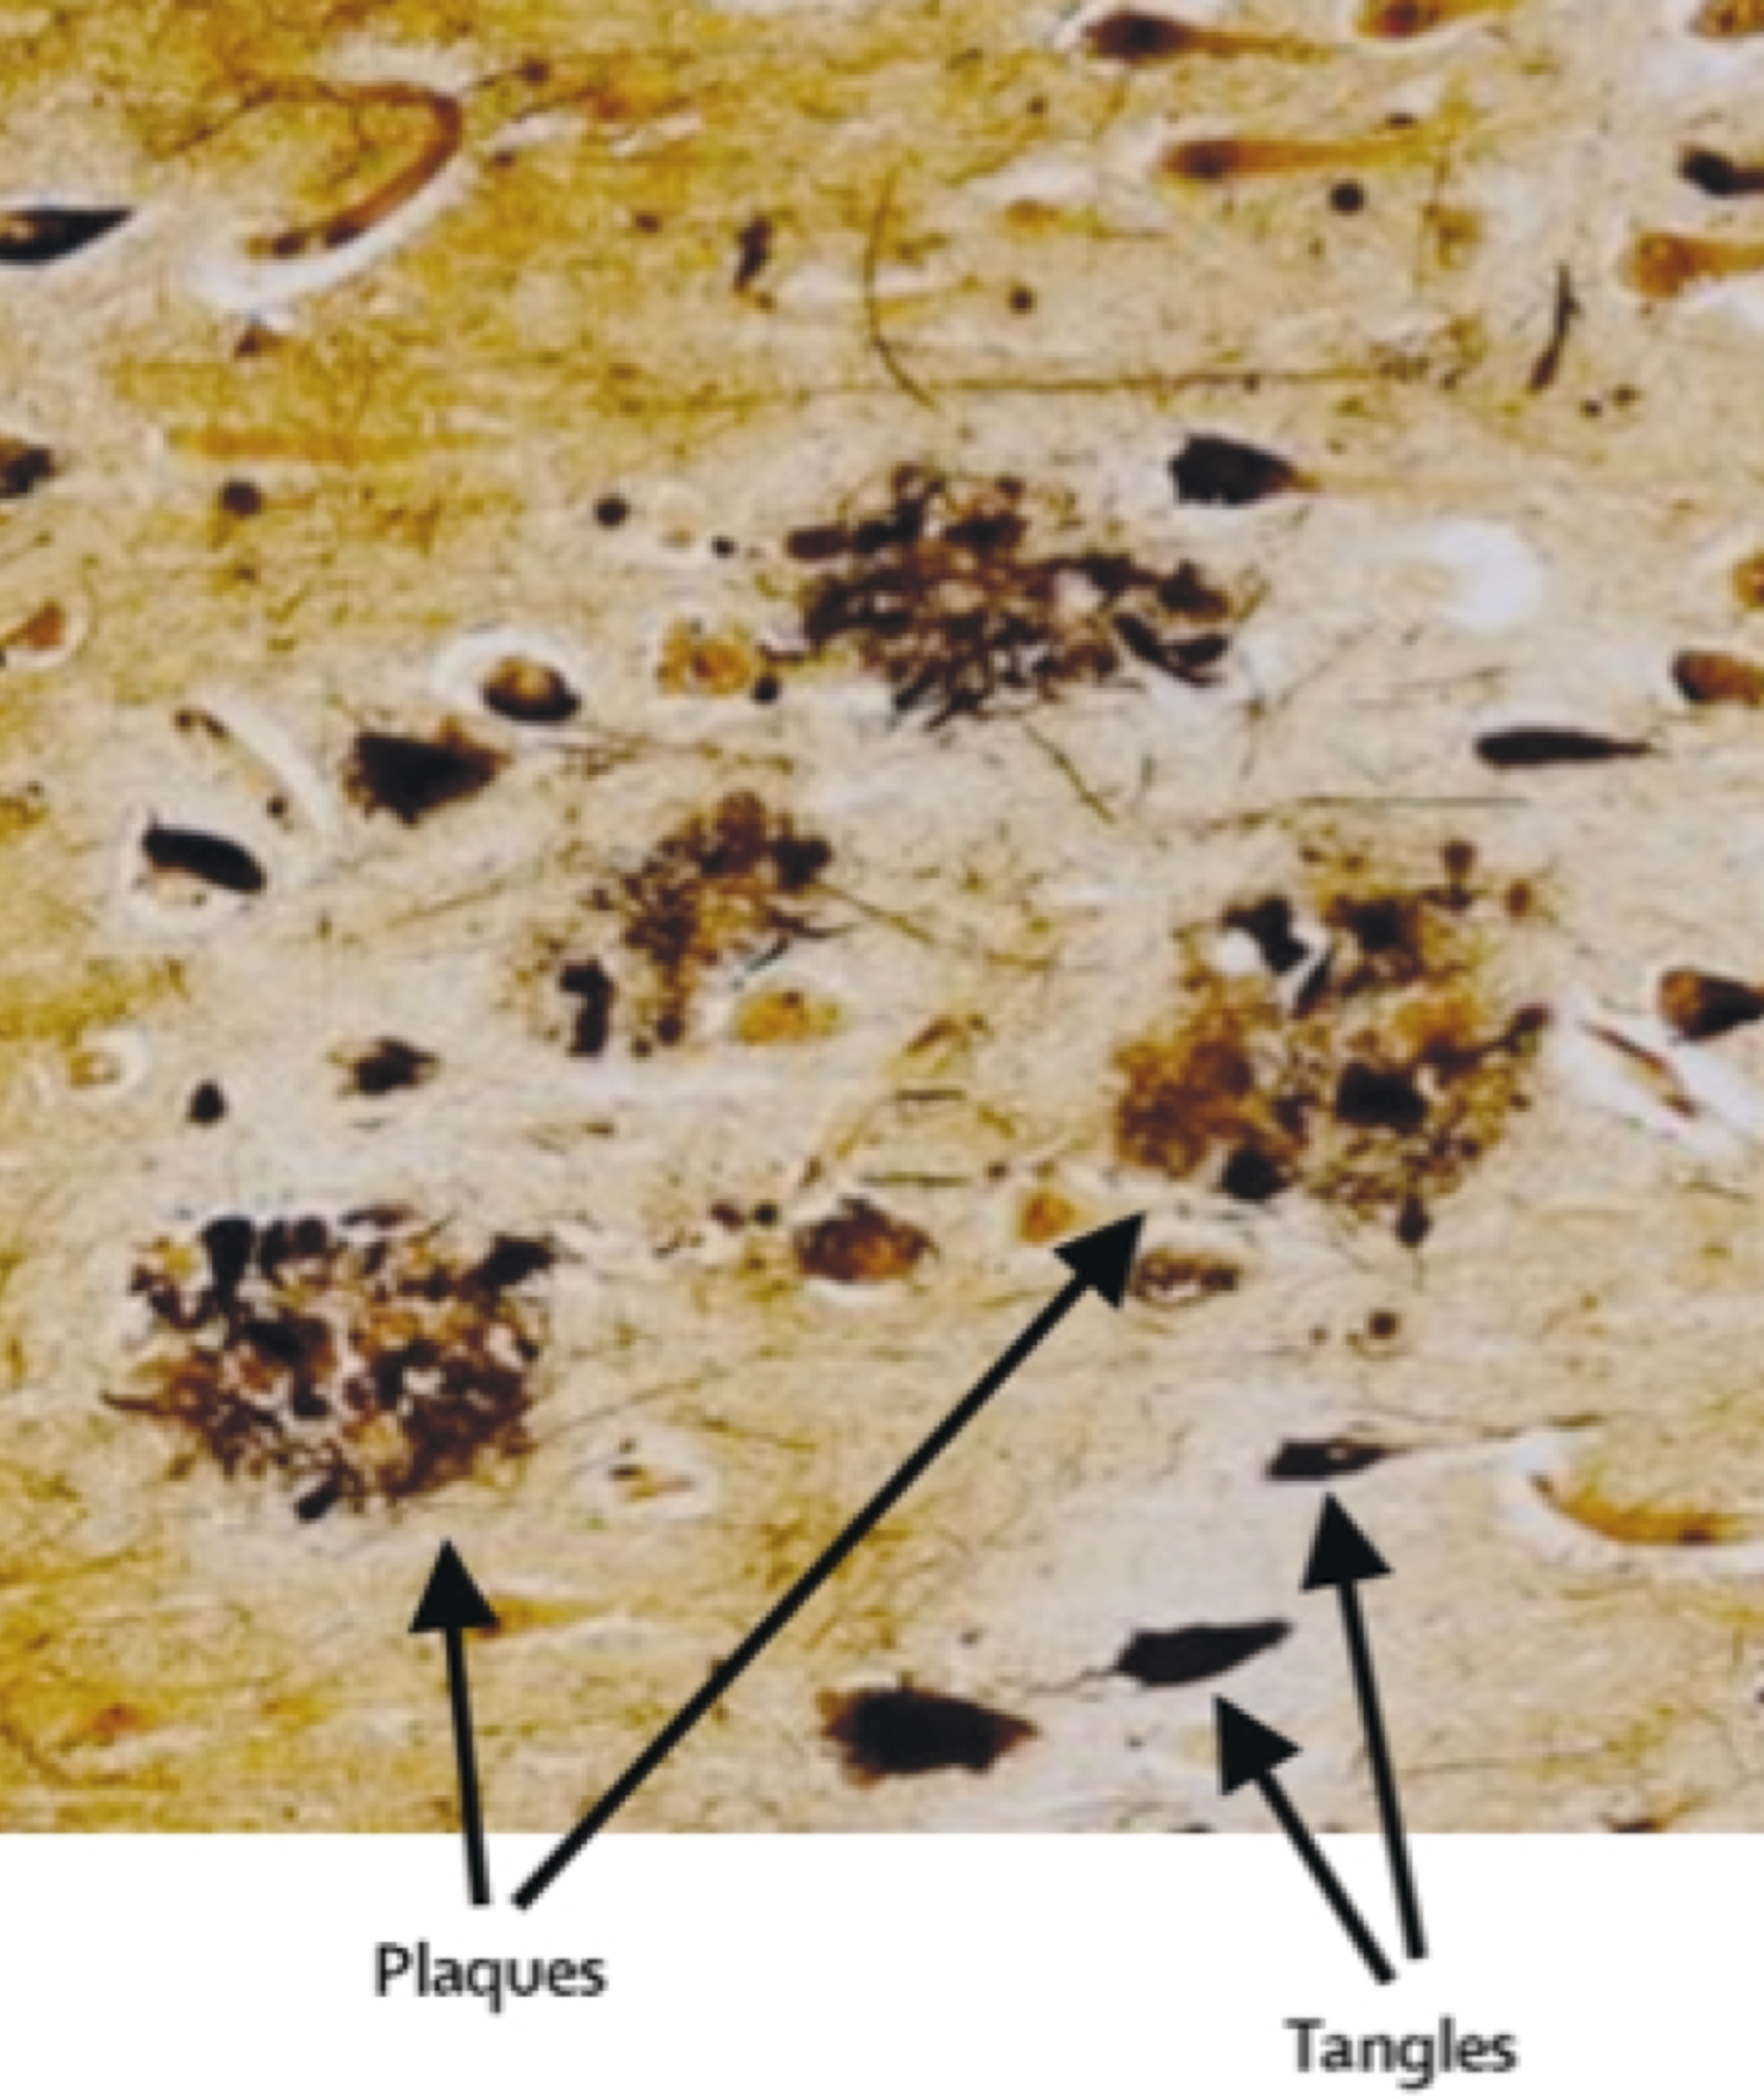
\includegraphics[width=6in]{figures/introduction/AD_tissue_pathology.pdf}
  \caption[Image of lesions formed by plaques and NFTs on brain tissue]{This is adapted from Blennow, 2006}
  \label{fig:AD_tissue_pathology}
\end{figure}

Upon examination, the brains of deceased AD patients show significant neuronal dystrophy.  Pathologically, AD is characterized by the presence of extracellular deposits of senile plaques and neurofibrillary tangles, which appear as lesions on stained neuronal tissue under light microscopy.(Figure~\ref{fig:AD_tissue_pathology})

Although it has been more than one hundred years since Dr. Alois Alzheimer first presented the association between the presence of neuronal plaques and the clinical symptoms of presenile dementia characteristic of Alzheimer's disease (AD), the exact relationship between the two is still under much contention.  It was not until in the 1980s, the protein \abeta\ was identified as the largest component of plaques. % How is Abeta produced ? Is it only involved in Abeta? What's the physiological role of Abeta?

The presence of amyloid plaque deposits in brains of deceased dementia patients led to the formulation of the long-standing amyloid hypothesis, which posits that amyloidogenesis of \abeta\ plays a key role in the initiation of AD. XXX

Although both plaques and NFTs appear together, many studies have indicated that NFTs plays a secondary role to \abeta\ in the pathogenesis of AD.
% More details on evidence which show that NFTs are not likely the causative species. Knock out mouse models ... mice do not develop AD, and instead develop tau pathologies  NFTs have also been shown to be affected by \abeta\ production.

% should I include more details on how Abeta is known to be produced in the body?
Monomeric \abeta\ is an approximately 4 kDa peptide produced by intramembrane proteolytic cleavage of the larger amyloid-$\beta$ precursor protein (APP) and is produced constitutively as part of the normal cellular metabolism.\{Selkoe, 2002 \#222\} APP is sequentially processed by the aspartyl proteases $\beta$-secretase and $\gamma$-secretase, where depending on the position of the cleavage by $\gamma$-secretase, a pool of \abeta peptides of lengths varying from 38 to 43 residues are produced. The peptides spanning residues 1-40 (\abetaforty) or 1-42 (\abetafortytwo) are predominantly found in AD-associated plaques. Neuritic plaques is composed of mainly \abetafortytwo, whereas \abetaforty\ is more commonly found in cerebralvascular plaques.

Multiple lines of evidence indicate that \abetafortytwo is likely to be the more deleterious form of \abeta. Genetic studies showed that mutations which cause early-onset AD also in turn increases the ratio of \abetafortytwo to \abetaforty.\cite{Hardy:1997tu} Moreover, in vitro, \abetafortytwo\ displays significantly higher propensity for aggregation than \abetaforty, despite differing by only two amino acids. In addition, \abetaforty\ and \abetafortytwo\ also have distinct aggregation pathways in vitro: \abetafortytwo is found to form a morphologically more diverse population of intermediate oligomers than \abetaforty.\cite{Bitan:2003ut}

% What about mice studies?

\abeta\ aggregates is present in a variety of morphologies in the brain. Although plaques are often visible in the dementia patients, the plaque load does not correlate with disease progression and severity, a puzzling aspect of AD.  Instead, synaptic loss correlated well with the concentration of soluble \abeta\ oligomers in the brain.

Currently there is a lack of treatment which targets the underlying disease. Most approved treatments today for AD only mitigates cognitive symptoms.  The vast number of structural and biochemical studies on amyloid structure have been crucial for the development of potential therapeutics for Alzheimer's disease.

%  Drug development for Alzheimer's has been on preventing amyloid aggregation and decreasing amyloid production. We will discuss this in more detail in later section XXX.
% Talk about how important it is to develop drugs for these amyloid disorders ... particularly for AD ... because it not only is a great economic burden on society, but a growing epidemic....

% \subsubsection{Other disorders}
% % Perhaps not enough to make it into its own subsection
% In addition to AD, other neurodegenerative diseases have been shown to involve the presence of amyloid.  Parkinson's disease, Huntington's, Prion disorders (Mad cow).  These diseases and their pathology are reviewed elsewhere and are beyond the scope of the thesis.
% I think I will not mention these things in detail in my introduction


\section{Amyloid Inhibition by small molecules: A promising method of treatment for AD}
% Cure, method of prevention; is there hope?

% In this section, I will provide an overview of some of the challenges to overcome when developing a small molecule therapeutic for Alzheimer's disease.  Furthermore, using this information, I will motivate why inositol is an exciting avenue to explore.

% Amyloid inhibition as a treatment for Alzheimer's disease and related amyloid disorders. 

% Briefly mention non-small molecule putative therapies which also acts via amyloid inhibition. The focus of this thesis will be on small-molecule amyloid inhibition.

% Use this as a transition into amyloid inhibition
% AD presents as a major economic and health burden to modern society.  With the longevity of our population, AD is approaching epidemic proportions with no cure or preventative therapy available.\cite{Blennow:2006wd}

Amyloids are attractive drug targets. Small molecules which targets amyloids may be an effective method of treatment for amyloid disorders because of the potential to treat the underlying disease. Through in vitro screening, many small molecules have been found to effect the amyloid aggregation pathway.  Some were demonstrated to inhibit amyloid fibrils, where as others were shown to arrest or reduce oligomer formation.
  
% Here I can take a cue from Justin Lemkul`'s recent review paper.
% Talk about the different kinds of small molecules that have been found to inhibition amyloid formation.  Here I will also provide a summary of what people know about the mechanism by which they inhibit amyloid formation.
Pharmacological perspective of the challenge of developing an Alzheimer's drug. In order to effectively treat Alzheimer's and other neurodegenerative diseases, small molecule drug candidates must pass the blood brain barrier at sufficient concentrations for inhibition.  This is difficult to achieve.
      
In vitro screening has led to the discovery of a large number of small-molecules which were found to affect the amyloid aggregation pathway. Many of these small molecules are thought to act by directly binding to amyloidogenic peptides and aggregates.

\begin{figure}
\centering
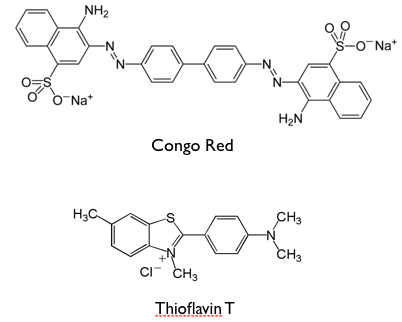
\includegraphics[width=3in]{figures/introduction/dyes.png}
\caption[Small molecule binders]{Amyloid binding dyes Congo Red and Thioflavin T}
\label{fig:amyloid_dyes}
\end{figure}

\subsection{Dye molecules}
Thioflavin T and Congo red are two dye molecules that are often used to identify the presence of amyloid fibrils.  

Early histological detection of amyloid binding was done using congo red, where upon binding fibrils exhibit red-green birefringence. Congo red requires the use of polarized light microscopy, a laborious process, and the interpretation of the birefringence is often not reproducible.

Thioflavin-T (ThT) is a benzathiole fluorescent dye also used to detect the presence of amyloid fibrils in post-mortem brain tissue samples, and monitor fibril formation in vitro. ThT exhibits a dramatic shift in the excitation spectrum maximum and an emission enhancement upon binding to fibrils, making it a sensitive and efficient report for the presence of amyloid fibrils.

Moreover, ThT is soluble in water and have \KD in the low \micromolar\ range.  ThT also binds uniformly across fibrils prepared from synthetic and biological sources.

The studies by Naiki et al. and LeVine showed that dye binding is linked to the presence of the \crossbs of fibrils, which led to the adoption of ThT dye binding as not only an indication of the presence of fibrils, but also as an indication of the presence of the \crossbs.

% Furthermore ThT fluorescence is only observed from those molecules that have bound to the fibrils.  
% ThT exhibits a shift in the excitation spectrum maximum, from 385 nm to 450 nm, and the emission maximum, from 445 nm to 482 nm

% This is from \cite{Wu:2011fd} which briefly summarizes why ThT binding gives rise to the excitation spectrum.
% These phenomena stem from two effects of binding.
% Firstly, steric and electronic stabilization (via charge trans- fer) of the ground-state charge distribution (7,8); and 2), restriction in the rotation of the aromatic rings of the dye (see Fig. 1 A) in its electronically excited state (9,10).



Both molecules appear to consistently bind mature amyloid fibrils.  Being \bsheet-rich does not imply that these dye molecules would bind. Also can affect fibril formation.(Fig.~\ref{fig:amyloid_dyes})

\begin{figure}
\centering
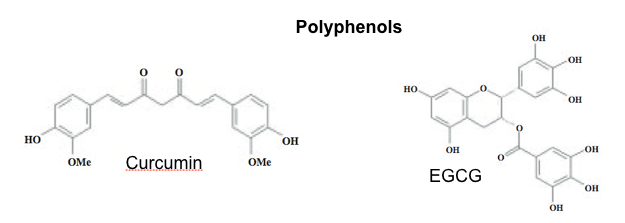
\includegraphics[width=6in]{figures/introduction/polyphenols.png}
\caption[Small molecule binders]{Polyphenols}
\label{fig:polyphenols}
\end{figure}

\subsection{Polyphenols}
Polyphenols,  is a large group of natural and synthetic molecules.  (−)-epigallocatechin-3-gallate, curcumin, and a polyphenolic grape seed extract, known for their anti-oxidant properties,  were recently discovered to be capable of affecting amyloid formation.(Fig.~\ref{fig:polyphenols})

\subsection{Inositol}
\begin{figure}
\centering
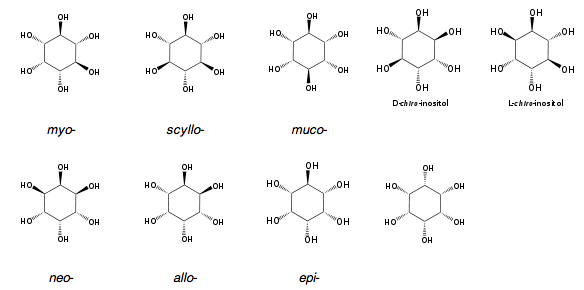
\includegraphics[width=6in]{figures/introduction/inositol.png}
\caption[Inositol]{Inositol stereoisomers}
\label{fig:inositols}
\end{figure}

% Should tell a little story of how inositol was discovered.  I remember that Chris Yip thought this might have been nice ... because it seems out of the blue to people.

% What I wrote in my transfer proposal:

Inositol with the molecular formula of \ce{C_6H_12O_6}, is a simple polyol with nine naturally occurring stereoisomers. Out of these nine isomers, seven are optically inactive, and the remaining two (L- and D-chiro-inositol) are chiral enantiomers.(Figure~\ref{fig:inositols})

% Here, use the physiological role of myo-inositol as a lead to transition into its role in amyloid inhibition.

Myo-inositol, the most abundant isomer, is ubiquitous in all eukaryotes and is a physiologically important osmolyte.  Furthermore, myo- is a precursor for inositol lipid synthesis: It is a constituent of phosphatidylinositol, an important phospholipid in membranes and second messenger systems. Once phosphorylated, myo-inositol phosphatides act as second messengers in intracellular signal transduction pathways.\cite{Fisher:2002tk}

Inositol is found in high concentrations in tissues of the human central nervous system (CNS): myo- And scyllo-inositol have approximate concentrations of 5 and 0.1-0.5 mM in the CNS, respectively.\cite{Fisher:2002tk} Accordingly, inositols also function as osmolytes in the CNS, where alterations in their concentrations are known to be associated with neuropathological conditions.\cite{Michaelis:1993gf, Fisher:2002tk}

% Role of inositol in amyloid inhibition. Here, include the background on how inositol was discovered as an \abeta\ amyloid fibril inhibitor
In recent years, scyllo-inositol have been identified as a promising therapeutic candidate for the treatment of Alzheimer's Disease.

Scyllo-, myo-, and epi-, but not chiro-inositol, have been shown to inhibit \abeta42 fibril assembly, stabilize an oligomeric complex of \abeta42, and attenuate \abeta-oligomer-induced neurotoxicity in vitro. Moreover, inositol exhibits stereochemistry-specific effects on \abeta\  fibril inhibition and cytotoxicity: scyllo- and epi- are more effective than myo-inositol, whereas chiro-inositol was inactive.\cite{McLaurin:2000bq}

An important therapeutic advantage of scyllo-inositol is its ability to readily crosses the bloodbrain barrier (BBB) (both actively and passively transported). Because it is not enzymatically broken down in the gut, it may be administered as a drug orally. 
% Inositol is synthesized inside the body ... or can be obtained via nutrition?  
		
In vivo studies with a transgenic mouse model of AD demonstrated that alleviation of symptoms after inositol treatment was correlated with a decrease in the levels of soluble \abeta\ oligomers, suggesting that the beneficial effects of scyllo-inositol may be attributed to the inhibition and/or disaggregation of high-order \abeta\ oligomers.\cite{McLaurin:2006eb}

Taken together, these results suggest that scyllo-inositol, and its derivatives, are a potential therapy for AD with the ability to change the course of the disease.\cite{Nitz:2008jl,Sun:2008ko}

% Include some data on human clinical trials (?) -- II was negative ... how to say it ? Should read phase II paper.
Presently scyllo-inositol completed both phase I and II of human clinical trials, where it was demonstrated that inositol is not toxic to healthy individuals at concentrations effective for amyloid inhibition.

\subsection{Commonalities between small molecule inhibitors}
% Commonalities between small molecules which appear to affect amyloid aggregation
Small molecule inhibitors share common chemical features and groups.  They are typically planar in geometry, have many aromatic rings, and polar functional groups (hydroxyl groups) around the edge of these aromatic rings.



\subsection{Molecular mechanisms of amyloid inhibition 
	            \\ by small molecules}
% Mechanism of action.
Some small molecules inhibit fibril formation, where as others may prevent oligomerization, but not fibrillation. A high concentration is often required to observe activity (micromolar to millimolar), which suggests that they may be non-specific inhibitors. EGCG, one such polyphenol, is known to have the lowest IC50.
    	% IC50 -- This quantitative measure indicates how much of a particular drug or other substance (inhibitor) is needed to inhibit a given biological process (or component of a process, i.e. an enzyme, cell, cell receptor or microorganism) by half.
      % EC50 -- The term half maximal effective concentration (EC50) refers to the concentration of a drug, antibody or toxicant which induces a response halfway between the baseline and maximum after some specified exposure time.[1] It is commonly used as a measure of drug's potency.
      % Ref: wikipedia
      
  	% Review of what is known about amyloid fibril ligand binding, specifically dyes.

Molecular mechanism of binding of dye molecules. Thought to bind flat on on the surface grooves of amyloid fibrils where they interact with hydrophobic groups exposed at the surface. 
      % Doesn't explain why the dye molecules are also able to suppress fibril formation.
      % Can the birefringence be explained by these binding modes? -- this is out of the scope of my thesis.  Don't put this in my thesis but I should be able to coherently explain this during my defense.

\section{Analogy to Sugar-protein binding}
% Does this section fit here? Where should I put it?
% Could use this as a prime example of protein-ligand interaction ...
% As a prime example of protein ligand interaction, one of the first systems that was used to understand binding was a sugar binding protein lysozyme ... -- No I think I will use early systems used to understand protein-ligand binding and if that was a sugar binding protein, then it will come off as a coincidence.
% This section is best discussed in the context of understanding inositol binding ...

% Mention some experimental techniques used to obtain protein sugar-binding modes, but the point here is not to review these methods ... but to point out that I am aware of these techniques.

\subsection{Sugar Binding modes}

% This section provides a nice lead in to the methods section
\section{Protein-ligand interactions}
\subsection{Forces involved in binding}
% Note that I may end up introducing the forces up in the earlier section -- reorganize as needed
\begin{outline}
	\1 Protein-ligand non-covalent interactions that are important for ligand binding and recognition
		\2 Electrostatic interactions. Polar (hydrogen bonding) and charge-charge interactions
		 % Here, it will benefit me to read Sarah's appendix C carefully.
		\2 Nonpolar (hydrophobic) interactions
		  \3 Van der Waals
\end{outline}

\subsection{Binding equilibria}
% subsection protein_ligand_binding_theory (end)
% Below is a summary of an excerpt from Tom's thesis on structure-based drug discovery.
% Design of antibiotics 
% 1) Target determination (biochemical)
% 2) Structural determination (Xray, NMR, or homology); active site identified; Here would be useful to get the holo structure of the protein
% 3) Screen for inhibitors against a chemical library or in silico docking.
\begin{outline}
	\1 Enzyme and its putative ligand typically bind specifically (high affinity binding).  We want to optimize binding specificity to increase the efficacy of the putative drug, and decrease adverse side effects (toxicity) in the human body.

	\1 The dissociation constant, $K_d$, is a measure of the affinity of a ligand for its binding site on the host protein. Pharmacologically, it can be interpreted as the concentration at which 50\% of the drug is bound to the protein. In experimental studies, $K_d$ is often used to quantitatively screen for potential drug candidates. 
  % A small $K_d$ suggests that the ligand may bind tightly to the protein.

	\1 Binding equilibrium

    \begin{equation}
      \left[ Protein\cdot Inositol \right] 
      \rightleftharpoons 
      \left[ Protein \right]+\left[ Inositol \right]
    \end{equation}
  
    % \2 Absolute binding free energy
    % \2 Relative binding free energy
    
	\1 The binding free energy of a ligand to a protein is directly related to its dissociation constant, $K_d$, the equilibrium constant of the above reaction

     \begin{equation}
        K_{d} = f_{ub}\frac{\left[ Protein \right]\left[ Inositol \right]}{\left[Protein \cdot Inositol\right]},
     \end{equation}
     
     % Add equation converting binding constant to gibbs free energies.
	\1 Experimental techniques for estimating $K_d$
		\2 What experimental techniques are used to estimate binding affinity? (May need to study up on this)
		\2 Isothermal titration calorimetry (ITC) is a technique which can be used to measure energetics of ligand binding to peptides.
\end{outline}

% \subsection{Role of chirality in drug binding}
% Stereoisomerism is important to the activity of molecules.  It modulates binding to proteins.
% Two types of stereochemistry
% Constitutional isomers - differs in bonding sequences and connectivity
% Stereoisomers - differs in orientation of their atoms in space, but no connectivity differences.
% Definition of chirality [Add schematic] ... etc
% Molecules with chirality have a non-superimposable mirror image, called an enantiomer.
% A carbon molecule with four different groups has chirality.

\section{Thesis objectives and rationale}
% Understanding amyloid inhibition in the context of the framework of traditional enzyme inhibition mechanism
\subsection{Challenges of amyloid inhibition}
\begin{outline}
       % However, most of these studies were focused on A$\beta$ and large A$\beta$ aggregates,\{Fawzi, 2008 \#553;Esposito, 2008 \#567;Sgourakis, 2007 \#609;Wei, 2006 \#656;Tarus, 2006 \#628 Karsai, 2006 \#658\} and thus, were computationally limited by the complexity of the molecular systems.

    \1 The protein-ligand binding model developed to understand enzyme inhibition cannot be directly applied to understand the molecular mechanism of amyloid inhibition by small molecules. 
    
      \2 Amyloid inhibitors are found to be very weak binders. How do non-specific inhibitors act as a drug? And how do we approach this with MD simulations?
      
      \2  Because the A$\beta$ amyloid aggregate pathway encompasses a variety of species, some of which has no folded structure, a single conformation cannot be assumed for binding. Furthermore, structural information of amyloidogenic species lags behind those of enzymes, which tends to be globular proteins amenable for X-ray crystallography. This means that the putative binding sites are not known.
      
      \2 The structural disorder of the peptides involved poses a challenge for obtaining converged properties from MD simulations. 
    
    	\1 A$\beta$ peptides are completely disordered.  We also do not know what the binding site looks like, where it is located on these structures.
    	
    \1 To date, few studies have attempted to provide statistically meaningful results pertaining to general mechanisms of protein self-aggregation and amyloid formation. Furthermore, despite the abundance of MD studies of A$\beta$, few studies have systematically examined the mechanism of action of small molecule inhibitors of amyloids

    \1 In AD, there is the added challenge of the drug being able to cross the brain barrier, while remaining non-neurotoxic.  What kind of drugs cross the BBB?  Typically hydrophobic drugs.
\end{outline}    

\subsection{Study Design and Rationale}
\begin{outline}
	\1 Here describe in detail how I designed my study to circumvent the challenges presented by the amyloid inhibition problem, and the limitations  of MD simulations. At this point, clearly explain and discuss my study design and rationale. (Fig.~\ref{fig:rationale})

  \begin{figure}
    \centering
    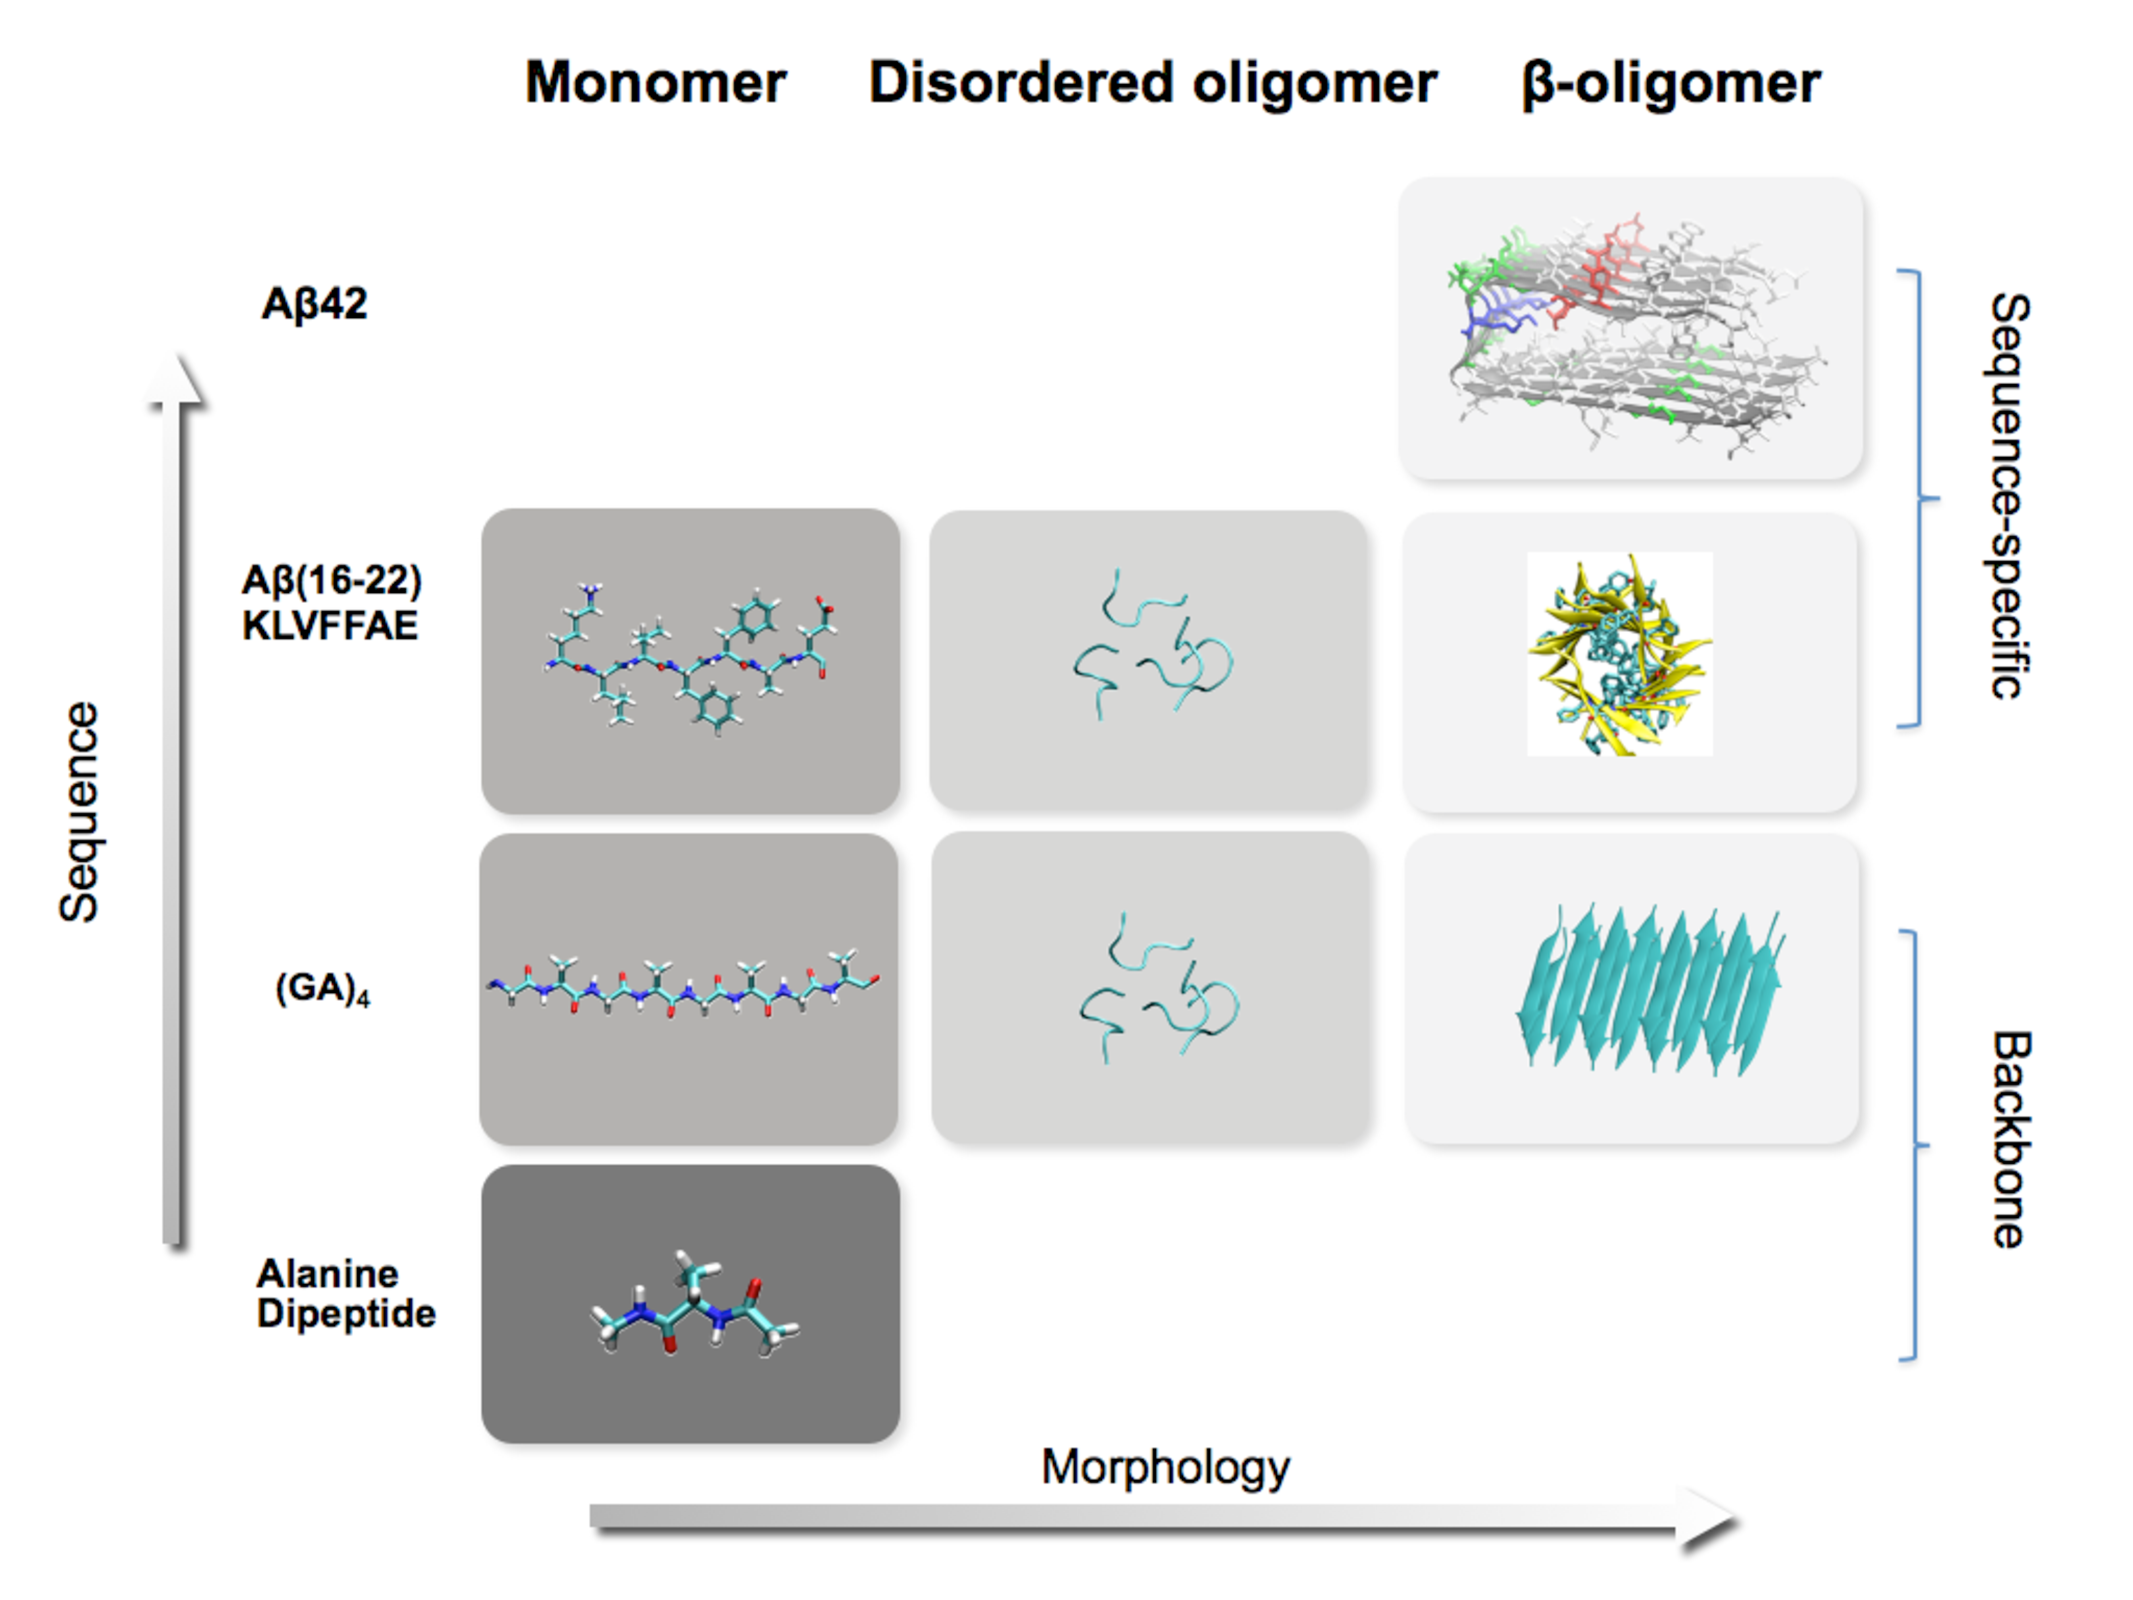
\includegraphics[width=6in]{figures/introduction/matrix.pdf}
    \caption[Rationale]{Shows the progression from small, model systems to larger and structurally more complex systems involving the full-length A$\beta$42 peptide.}
    \label{fig:rationale}
  \end{figure}

	\1 Beginning with the simplest model systems for an amyloidogenic peptide, the alanine dipeptide, we systematically examine binding of inositol with systems of both increasing sequence and structural complexity.

	% Use brute force simulations
	\1 We exploit conventional MD simulation techniques because simulation approaches used for understanding enzyme-ligand binding is not applicable. 
	
	\1 Instead, we use conventional MD simulations and repeats of independent simulations to determine the binding modes, and binding equilibria of inositol with amyloidogenic peptides and aggregates of A$\beta$.
\end{outline}

\section{Thesis Organization}
The first chapter introduces the thesis in the context of the field.  The second chapter introduces the main methods used in the work in the thesis. Chapters 3, 4, and 5 are the results of simulations of inositol with amyloid like peptides and aggregates. Chapter 6 shows work of the general applicability of our methods developed throughout this thesis to MD simulations to understand protein - carbohydrate binding. Chapter 7 provides discussion, suggestions for future work, and perspectives.

\addcontentsline{toc}{section}{Bibliography}
\bibliographystyle{plain}
\bibliography{chapter1}

% AD
% Treatment - harder to treat - lack of biochemical understanding of what causes disease, which makes it difficult to develop drugs for; lack of good diagnostic methods because treatment may not be effective at end stages of the disease where brain function won't e able to be rescued.
% Diagnosis - hard to diagnose
% AD is difficult to diagnose.  It is often not apparent that someone has AD until they exhibit symptoms severe enough to interfere with daily life or occupation. 

% Amyloid hypothesis - our best guess at what causes AD and provides the best guess at what we should be targeting. 
% Abeta Amyloid thus far provides the best clue to the molecular basis of AD, and thus a promising pathway to a cure for AD.

% In some individuals without dementia symptoms may have as much plaque as another with severe AD. Synaptic loss can be used as a measure of disease progression. 

% Perhaps use this as a transition into the general discussion of amyloid formation and structure -- not only specific to Abeta.
% Furthermore, amyloid have also been known to play beneficial roles in certain living systems. REF
% Increasing awareness of the amyloid state of proteins, and interest grew in amyloids because of their role in a variety of devastating human diseases.

% Fibrils

% In this section I will talk about how amyloid aggregation is thought to work. Introduce the thermodynamic model for understanding fibril formation.

% Model peptides
\chapter{Chapter 2}

Lorem ipsum dolor sit amet, consectetur adipiscing elit. Proin tellus nunc, accumsan sit amet blandit nec, accumsan a libero. Praesent blandit erat ut tellus congue eu facilisis leo malesuada. Nullam sit amet fermentum erat. Nunc mi leo, rutrum in tincidunt sit amet, imperdiet a nisl. Donec pulvinar, risus vel hendrerit elementum, lacus eros fringilla est, sed condimentum massa libero ac velit. Donec non sapien nunc, eget pellentesque lectus. Maecenas est quam, convallis non sagittis at, accumsan id risus. Duis gravida faucibus nisi auctor rutrum. Vestibulum rutrum massa in orci iaculis a condimentum nisl accumsan. Donec placerat, turpis et rutrum facilisis, nisl turpis condimentum nibh, a adipiscing massa elit non lorem. Quisque et nisl vel lectus tincidunt pulvinar quis eget arcu. Donec erat neque, malesuada sed euismod vel, tempus quis purus. Mauris dictum mauris ante. Class aptent taciti sociosqu ad litora torquent per conubia nostra, per inceptos himenaeos.

Pellentesque vitae nulla a nisi tincidunt scelerisque et in justo. Aenean et urna sed enim luctus interdum sed et magna. Phasellus eget orci ac nulla consectetur porta a eget felis. Aenean egestas lorem vel nulla suscipit mollis. Cras interdum, elit at aliquam commodo, purus risus aliquam mi, sit amet tempus neque mi a dui. Nulla ante est, porta eget adipiscing sit amet, mollis a purus. Etiam sit amet ultrices nisi. Lorem ipsum dolor sit amet, consectetur adipiscing elit. Nunc ultricies odio non dolor condimentum viverra.

Maecenas ac lectus sed velit convallis auctor. Nullam ultrices augue ut arcu rhoncus pellentesque rutrum lectus blandit. Maecenas lorem elit, interdum eget egestas ac, ultrices a enim. Sed sodales nunc a lectus interdum non faucibus nunc ornare. Curabitur varius porttitor quam, congue elementum urna tristique in. In et magna libero, at pretium augue. Nunc scelerisque egestas justo non mollis.

Fusce in augue lacus, vitae rhoncus nisl. Nulla mattis imperdiet luctus. Praesent est magna, eleifend nec accumsan vel, sodales in leo. Maecenas augue urna, aliquam a iaculis eu, tincidunt ac dolor. Integer vitae augue tellus, in porta diam. Cras sit amet condimentum justo. Etiam mollis leo vel tortor dignissim ac varius est rutrum. In quis libero purus, quis sagittis risus. Cras imperdiet dapibus posuere. Nulla gravida molestie ligula eget mollis. Vivamus facilisis viverra leo, in tincidunt urna imperdiet et. Aenean turpis eros, pharetra eget faucibus at, eleifend eget neque. Duis augue nisi, hendrerit in malesuada nec, aliquet quis dolor. Donec ut condimentum est. Nunc ac lorem at diam dictum sodales ac vitae diam.

Quisque sollicitudin nisl ac turpis consequat ut ultrices massa adipiscing. Ut tempor ligula ut est elementum et elementum nulla imperdiet. Aliquam id gravida ligula. Praesent vel nibh felis. Aliquam mollis nisl in nibh dictum at mollis turpis tristique. Curabitur vitae risus sapien, et fermentum lectus. Mauris eleifend ornare neque sit amet condimentum. Proin turpis nisi, mollis eu pretium ac, dictum et eros. Proin eu lorem quis leo cursus pretium. Praesent nunc metus, euismod at lacinia id, pharetra adipiscing dui. In hac habitasse platea dictumst.

Lorem ipsum dolor sit amet, consectetur adipiscing elit. Proin tellus nunc, accumsan sit amet blandit nec, accumsan a libero. Praesent blandit erat ut tellus congue eu facilisis leo malesuada. Nullam sit amet fermentum erat. Nunc mi leo, rutrum in tincidunt sit amet, imperdiet a nisl. Donec pulvinar, risus vel hendrerit elementum, lacus eros fringilla est, sed condimentum massa libero ac velit. Donec non sapien nunc, eget pellentesque lectus. Maecenas est quam, convallis non sagittis at, accumsan id risus. Duis gravida faucibus nisi auctor rutrum. Vestibulum rutrum massa in orci iaculis a condimentum nisl accumsan. Donec placerat, turpis et rutrum facilisis, nisl turpis condimentum nibh, a adipiscing massa elit non lorem. Quisque et nisl vel lectus tincidunt pulvinar quis eget arcu. Donec erat neque, malesuada sed euismod vel, tempus quis purus. Mauris dictum mauris ante. Class aptent taciti sociosqu ad litora torquent per conubia nostra, per inceptos himenaeos.

Pellentesque vitae nulla a nisi tincidunt scelerisque et in justo. Aenean et urna sed enim luctus interdum sed et magna. Phasellus eget orci ac nulla consectetur porta a eget felis. Aenean egestas lorem vel nulla suscipit mollis. Cras interdum, elit at aliquam commodo, purus risus aliquam mi, sit amet tempus neque mi a dui. Nulla ante est, porta eget adipiscing sit amet, mollis a purus. Etiam sit amet ultrices nisi. Lorem ipsum dolor sit amet, consectetur adipiscing elit. Nunc ultricies odio non dolor condimentum viverra.

Maecenas ac lectus sed velit convallis auctor. Nullam ultrices augue ut arcu rhoncus pellentesque rutrum lectus blandit. Maecenas lorem elit, interdum eget egestas ac, ultrices a enim. Sed sodales nunc a lectus interdum non faucibus nunc ornare. Curabitur varius porttitor quam, congue elementum urna tristique in. In et magna libero, at pretium augue. Nunc scelerisque egestas justo non mollis.

Fusce in augue lacus, vitae rhoncus nisl. Nulla mattis imperdiet luctus. Praesent est magna, eleifend nec accumsan vel, sodales in leo. Maecenas augue urna, aliquam a iaculis eu, tincidunt ac dolor. Integer vitae augue tellus, in porta diam. Cras sit amet condimentum justo. Etiam mollis leo vel tortor dignissim ac varius est rutrum. In quis libero purus, quis sagittis risus. Cras imperdiet dapibus posuere. Nulla gravida molestie ligula eget mollis. Vivamus facilisis viverra leo, in tincidunt urna imperdiet et. Aenean turpis eros, pharetra eget faucibus at, eleifend eget neque. Duis augue nisi, hendrerit in malesuada nec, aliquet quis dolor. Donec ut condimentum est. Nunc ac lorem at diam dictum sodales ac vitae diam.

Quisque sollicitudin nisl ac turpis consequat ut ultrices massa adipiscing. Ut tempor ligula ut est elementum et elementum nulla imperdiet. Aliquam id gravida ligula. Praesent vel nibh felis. Aliquam mollis nisl in nibh dictum at mollis turpis tristique. Curabitur vitae risus sapien, et fermentum lectus. Mauris eleifend ornare neque sit amet condimentum. Proin turpis nisi, mollis eu pretium ac, dictum et eros. Proin eu lorem quis leo cursus pretium. Praesent nunc metus, euismod at lacinia id, pharetra adipiscing dui. In hac habitasse platea dictumst.


% % KLVFFAE
% \include{results-chapter-2}
% 
% % Abeta42
% \include{results-chapter-3}
% 
% % PGab
% \include{results-chapter-4}
% 
% % Discussion / Perspectives
% \chapter{Perspectives, Conclusions and Future Directions}
% Example sentences found in teh conclusions and summary chapters of people's thesis 
% The work presented in this thesis has ...

% Because this work represents the first atomistic simulation, to our knowledge, demonstrating that polypeptide chains can form entangled polymer melt-like states, it contributes to an improved understanding of both elastin coacervation, and the more general phenomenon of protein aggregation

% Everyone's conclusions all had a significant amount of Future directions. (~3 pages worth)
% Strategy:  take the conclusion paragraphs of each chapter and then meld it into a conclusions chapter.

% Make a clear and concise statement of the original contribution to knowledge found in your thesis.

%What has this work led to?
%This has led to the understanding of mechanism of amyloid formation.
%An exploration of carbohydrate binding.


% One sentence summarizing AD and the medical challenges that it poses.  Summarize why it is difficult to design a drug for AD. 
% Summary of the core technique that is used in this thesis
Alzheimer?s Disease (AD) is a devastating neurodegenerative disease that is the most common cause of dementia in persons of age 65 or older. Currently there is no cure or method of treatment that targets the underlying disease.  As the world's population is living ages, AD will reach epidemic levels and will pose a tremendous medical burden for society. The overall goal of this thesis work is to investigate the molecular basis of amyloid inhibition by inositol, a small-molecule putative therapeutic for the treatment of Alzheimer's disease. By utilizing molecular dynamics simulations, a computational technique based on classical physics which allows us to simulate the motions of physical systems at the atomistic-level, we systematically examine model amyloidogenic peptides and aggregates to more complex systems involving the full-length A$\beta$42 peptide. The work presented in this thesis contributed to 2 peer-reviewed articles and 2 manuscripts in preparation which form the basis of Chapters 3 to 6.  The key results from each of these chapters are summarized below.

Beginning in chapter 2, I performed systematic simulations of simple amyloidogenic peptide models with scyllo- and chiro-inositol, stereoisomers of inositol, to examine the role of backbone binding on amyloid inhibition. My results indicated that although peptide backbone dominates the interaction with inositol, the binding affinity is low and remains in the millimolar range. Moreover, this property is independent of stereochemistry and does not appear to be sufficient to impede peptide dimerization through intermolecular backbone hydrogen bonding. Taken together, my results in this chapter suggest that amyloid inhibition by inositol cannot be accounted for by generic binding to the peptidic backbone alone. Rather, it is likely to involve sequence-specific interactions with amino-acid side chains as well as binding to specific aggregate morphologies.
% Accordingly, although the formation of intermolecular hydrogen bonds is the predominant interaction in protein aggregates composed of \gafour, amyloidogenic peptides involved in amyloid diseases are often more hydrophobic and in general, self-aggregation is driven largely by the hydrophobic effect.\cite{Chiti:2006p20}

To further investigate the role of sequence-specific interactions between inositol and aggregates of pathogenic peptides, I examined the binding of  inositol stereoisomers, successively to monomers, disordered oligomers, and $\beta$-sheet aggregates of A$\beta$(16-22), whose sequence is thought to be the core aggregation region in the A$\beta$42 peptide (chapter 4). A key finding of this study was that the $K_{eq}$ of inositol ($\sim$0.2 - 0.5 mM) for the $\beta$-oligomer is commensurate with the concentration at which inhibition of amyloid formation by A$\beta$42 is observed \emph{in vitro}. Although both \emph{scyllo}- and \emph{chiro}-inositol exhibit similar binding affinities with all peptide states considered, my simulations have uncovered a stereospecific face-to-face stacking stacking mode of \emph{scyllo}-inositol with the Phe side chains and a higher propensity for hydrogen bonding, which together suggests a molecular basis for measured differences in activity. \textbf{Cooperative binding modes of inositol at grooves on the surface of the $\beta$-oligomer of A$\beta$(16-22) suggest a possible mechanism of fibril inhibition whereby inositol prevents the lateral association or stacking of protofibrillar $\beta$-sheet oligomers.} Furthermore, my results suggest that the fibril core of A$\beta$ amyloid aggregates contains carbohydrate-like binding sites.  \textbf{As such, carbohydrate-based small-molecule derivatives may be a promising avenue to explore for the rational design of novel therapeutics for AD.}

In chapter 4, I investigate the binding of inositol to the protofibrillar form of A$\beta$42, the full-length peptide. Here, I found that there were no differences in the fibril conformations with and without inositol in either low or high molar ratio. 
% Does glucose bind more or less? If it does bind less, then it tells us that we might be onto something with scyllo-inositol even though the structure is subtly different.  
% Not sure what I meant here
Glucose does not necessarily bind ``less", but it does not bind on the right face ie. the KLVFFAE face Scyllo-inositol appears to preferentially bind the KLVFFAE face, more than glucose and chiro-inositol.  Furthermore, scyllo-inositol does not bind in a hydrated tunnel formed in the protofibrillar aggregate, where as both chiro-inositol and glucose Binding mode differences between active and inactive inhibitors of Abeta suggest a mechanism of inhibition.

In chapter 5, I demonstrated the generality of the methodology that was developed to study the binding mechanism of inositol by using a similar approach to study carbohydrate-protein binding. Specifically, ....  

\section{Significance for drug development for AD}
%[Thesis significance - part of the summary of what I make of my thesis ] 

There are a multitude of challenges in understanding the mechanism of a drug for treating neurodegeneration

This thesis demonstrates the applicability of MD simulations in providing insight into how drugs might bind to amyloidogenic species and intrinsically disordered peptides.  The results in this thesis can be used to map out a pharmacophore for developing a drug for the treatment of Alzheimer's Disease, opening the way to computer-aided design of improved diagnostics and therapeutics. A pharmacophore is an abstract description of molecular features which are necessary for molecular recognition of a ligand by a biological macromolecule - If I have to define this here, then it should have been in the introduction. \textbf{Definition is taken from the wiki.}

% Speculate on the future of drug development for AD in regards to the significance of thesis wrt curing AD. Will blocking aggregation work for AD? - May be this should in the introduction instead.
% (WRITE SOME CONCLUSIONS HERE … RELATING TO HOW A SINGLE SMALL MOLECULE BINDS SPECIFIC MORPHOLOGICAL STRUCTURES -- clearly a key result of my works demonstrate that there is sequence specificity) 

Because AD may be caused by a multitude of pathological changes in the brain, it is likely that a cocktail of compounds, each targeting a different disease pathway, may be required for treating AD. % (Adapted from pharmacophore for AD 2011)

% \section{MD simulations and Rational drug design}
\section{Contribution to sugar-protein binding}
% MD simulation as a tool for probing weak interactions
The work presented in this thesis have demonstrated that the methodology used in this thesis may be generally applicable to understanding carbohydrate-protein interactions. In chapter 4, we used simple sugars glucosamine and GlcNAc to map out a binding surface on PgaB, a protein invovled in the biofilm formation pathway. 

My work has demonstrated that MD simulations in combination with the use of current force fields can be effectively used to probe weak and transient molecular interactions, which are often not readily detectable using experimental techniques. One prominent example where weak interactions are prominent in protein-ligand binding is protein-carbohydrate interactions.\cite{weak binding review paper}

Understanding protein-sugar interactions is an important endeavor because of antibody binding to proteins.  Viruses often express carbohydrates on their coats.  Inhibiting bacterial action involves knowing how polysaccharrides are expressed, which involves binding proteins.  The results of this thesis presents methods that may be useful for developing antibiotics. \textbf{Rewrite this part to reflect and tie into how my work, methods, and how they are related to solving these problems} 

% The role of simulations in drug discovery to effectively predict binding modes and binding sites

[Thesis significance; more perspectives] Traditionally computation studies probing protein-ligand binding is often carried out with the knowledge of a putative binding site (often determined by X-ray crystallography) and the mechanism is examined employing sophisticated methods using the ligands thought to be able to bind in this specific pocket, while ignoring all other possibilities.  However, with the computing power to extend simulations to a longer time scale, MD simulations may be accurate in discovering new binding sites (even sites that are XXX high in affinity) without prior assumptions about the binding site. Our studies are among those which demonstrate the utility of MD to probe for binding sites that are difficult to obtain via experimental structural determination methods.  A recent MD study have demonstrated the capability of MD in binding site prediction for a folded protein.\cite{Shan:2011bo}

% Shan, 2011 (the DE shaw letter) An emerging challenge in drug discovery concerns the identification of allosteric ligand-binding sites (I’m not entirely convinced yet that this is important -- because I can’t think of any situations where this might be important -- convince myself or just drop this idea), through which drugs can modulate the effects of ligands that bind at the primary site.  More generally, an important limitation of traditional virtual drug screening is that it must start with a well-defined binding site (look into limitations of current drug discovery processes … may give some clue for constructing an argument for how MD is helping …), despite promising recent developments.\cite{Hetenyi, C.; van der Spoel, D. FEBS Lett. 2006, 580, 1447. (11) Davis,I.W.;Raha,K.;Head,M.S.;Baker,D.ProteinSci.2009, 18, 1998. }

\section{Significance for disordered binding}
% [Conclusions - A general interest in the specific work that I have done here ] 
Aside from contributing to the design of future AD therapeutics, our results have also contributed to the understanding of small molecule binding to disordered peptides (IDPs) in general. This is important because disordered binding are ubiquitous in biology, and disordered peptides and proteins and involved in many diseases such as X, Y, Z.  

Understanding how small molecules may interact with intrinsically disordered proteins goes beyond amyloid-related disorders. As IDPs are involved in many signalling pathways, they are also viable drug targets for many diseases.   Hence, targeting these disordered peptides using small molecules may be a possible therapeutic approach. For example, c-Myc is frequently involved in many cancers, \textbf{FILL IN THE GAP ABOUT HOW IT WORKS} and thus disruption of the c-Myc–-Max interaction is a possible anticancer strategy.\cite{Iakoucheva:2002uv,Metallo:2010p6822,Cuchillo:2012bm}

The work presented in chapters in this thesis sheds light on the mechanism of binding disordered peptides, and represents a step forward in understanding how small molecules may prevent protein - protein interactions, which involves identifying the binding interfaces, and understanding how to target these interfaces using small molecules.REFs.

\section{Osmolyte effects, denaturation, and macromolecular crowding}
% Note this is another hairy field … and you might want to stay the hell away from it, despite the fact that your thesis is loosely connected to this field
Another field of interest where weak interactions dominate is cosolvent effects on peptide folding. Simulations are a good use for probing that.  For example, MD simulations have been useful in gaining insight into protein denaturation mechanisms by urea or guanidinium, and the activity of osmolytes. Many of these are still open questions.\cite{http://pubs.acs.org/doi/abs/10.1021/jp200625k -- crowding and protein association.} Where am I going with this?

% These ideas below are  lesser developed ideas … consider cutting or bulk up …
% \section{other areas that are related to my work}
% [Ab-GAG membrane binding] This branches off the fact that I looked at sugar binding with peptides - amyloids when deposited may interact with glycosaminoglycans (part of the extracellular matrix) exposed at cellular surfaces. So what about it? Is my work helping to understand how amyloids are interacting with GAGs? or what role GAGs might play in accelerating amyloid formation?


% \subsection{Relationship to Polypharmacology -- where one drug binds to different targets?}
% Not sure how my thesis relates to this.

% I think this section is too crazy - eliminate.
%\section{In the future - perspectives on computer simulations}
% TODO: Find out why are there so few new drugs being discovered nowadays?
% Expand simulations into the macroscopic level 

% TODO: A good thought experiment - If I had the perfect simulation system? Predictive force field, simulate milliseconds in days.  How could I use this simulation system? Some effective use of the data? 

%Software has the ability to revolutionize drug discovery and take it from bench to personalized medicine. Molecular simulations can play a role in driving experimentation by helping to generate testable hypotheses.
%
%Virtual drug screening method using MD simulations as a component predicting drug toxicity.
%
%Here I'm speculating what the future of MD simulations might be ... A bit like science fiction with a touch of reality.
%
%Most Useful to “somehow” integrate experimental data with simulations results\cite{that nature paper discussing integrating MD and systems biology}
%- What are some success stories?
%what’s the real problem with drugs?
%Can we do without drugs? What are the therapies available?
%Small molecule
%peptide
%antibodies
%gene therapy (viral)
%\cite{Hansen:2012hh}

\section{Future directions}
% Better methods? Longer simulation times? Better force fields to detect hydrophobic effect?
% Better understanding of the amyloid aggregation mechanism will lead to a better understanding of the inhibition mechanism.

These are significance points.  Tie them better Studying different aggregate forms is useful.  One major conclusion of this thesis is that doing comparative systematic simulations is needed and useful for understanding the molecular basis of amyloid inhibitors how work.
[sketchy and would require a fast compute cycle -- look into more literature to formulate this idea better] This thesis shows that MD may be useful in the rational design of amyloid inhibitors from a template inhibitor. Molecular information obtained from simulations can be used to help design new derivatives, and simulations can be run for these chemically-modified forms of derivatives. 

\subsection{Simulations for other peptides involved in amyloid disorders}
Hard disk space and cpu power can be easily secured.  It would be a minor point to get that done.  Since there are many amyloid-associated disorders. In the future, simulations can be performed with these peptides while using a similar methodology. 

\subsection{Effect of inositol in the presence of lipid membranes}
Effect of the drug in the presence of lipid membranes => How does it affect aggregation in the presence of membranes. Does it prevent peptides from binding to the membrane?

\subsection{Apply enhanced sampling methods to study amyloid inhibition}
Extend simulations. The goal is to be able to simulate the entire aggregating process.  But this is not feasible because the timescale of fibril formation can take up to days. But can simulate the early stages of amyloid formation.  Use of enhanced sampling methods for aggregates in the presence of the drug.  These methods can enhanced Replica-exchange.  These methods enhance sampling and can speed up beta-sheet formation. With longer simulation times, can reach beta-sheet formation for shorter peptides such as KLVFFAE, we can add inositol (or some other drug) to understand their activity in early amyloid formation.


\section{Limitations}
Length of the peptides

\textbf{Lack of experimental data.} Finally, it would important to combine simulations with experimental studies.  This is a deficiency of this study. Simulations can be a good tool when combined with experimental validation by using a variety of techniques SSNMR and other biophysical techniques used to probe amyloid systems. Several studies are beginning to do that to understand the molecular mechanism of small molecule inhibitors ECGC.  In recent years several studies have begun to do this with some successes.





% How to separate references?
% Combined bibliography ? 

% Combine Methods -- how ?

%% This adds a line for the Bibliography in the Table of Contents.
\addcontentsline{toc}{chapter}{Bibliography}
%% ***   Set the bibliography style.   ***
%% (change according to your preference)
\bibliographystyle{plain}
%% ***   Set the bibliography file.   ***
%% ("thesis.bib" by default; change if needed)
\bibliography{thesis}

%% ***   NOTE   ***
%% If you don't use bibliography files, comment out the previous line
%% and use \begin{thebibliography}...\end{thebibliography}.  (In that
%% case, you should probably put the bibliography in a separate file
%% and `\include' or `\input' it here).

\end{document}

%%%%%%%%%%%%%%%%%%%%%%%%%%%%%%%%%%%%%%%%%%%%%%%%%%%%%%%%%%%%%%%%%%%%%%
%%  End of UT-THESIS.TEX
%%%%%%%%%%%%%%%%%%%%%%%%%%%%%%%%%%%%%%%%%%%%%%%%%%%%%%%%%%%%%%%%%%%%%%
